% ClearHPGL User's Manual
% Copyright (c) 2026 Adam G. Sweeney. Text written to ASD-STE100 and edited
% to The Chicago Manual of Style, 18th edition.
%
% Build (Tectonic, XeTeX engine):  tectonic clearhpgl-manual.tex
% ClearHPGL User's Manual: shared preamble.
% Build: tectonic clearhpgl-manual.tex
\documentclass[11pt,twoside,openright]{book}

\usepackage[letterpaper,inner=1.15in,outer=1in,top=1in,bottom=1.05in,
            headheight=14pt,headsep=0.3in]{geometry}

% ---- fonts (XeTeX through Tectonic) ---------------------------------------
\usepackage{fontspec}
\usepackage{unicode-math}
\setmainfont{texgyrepagella}[
  Extension=.otf, UprightFont=*-regular, BoldFont=*-bold,
  ItalicFont=*-italic, BoldItalicFont=*-bolditalic, Ligatures=TeX]
\setsansfont{texgyreheros}[
  Extension=.otf, UprightFont=*-regular, BoldFont=*-bold,
  ItalicFont=*-italic, BoldItalicFont=*-bolditalic, Ligatures=TeX]
\setmonofont{DejaVuSansMono}[
  Extension=.ttf, UprightFont=*, BoldFont=*-Bold,
  ItalicFont=*-Oblique, BoldItalicFont=*-BoldOblique, Scale=0.84]
\setmathfont{texgyrepagella-math.otf}

\usepackage{microtype}
% Code words cannot hyphenate; let a line stretch instead of overflowing.
\setlength{\emergencystretch}{3em}

% ---- color, boxes, figures ------------------------------------------------
\usepackage{xcolor}
\definecolor{navy}{HTML}{1B2F4B}
\definecolor{steel}{HTML}{3D5A80}
\definecolor{teal}{HTML}{2A9D8F}
\definecolor{amber}{HTML}{C77700}
\definecolor{signal}{HTML}{B3261E}
\definecolor{noteblue}{HTML}{1F6FB2}
\definecolor{codebg}{HTML}{F5F7FA}
\definecolor{rulegray}{HTML}{C9D1DB}
\definecolor{commentgreen}{HTML}{4E7A55}
\definecolor{stringred}{HTML}{9A3324}

\usepackage{graphicx}
\graphicspath{{figures/}}
\usepackage{tikz}
\usetikzlibrary{positioning,arrows.meta,shapes.geometric,shapes.misc,calc,fit,backgrounds,decorations.pathreplacing}
\usepackage[most]{tcolorbox}

% ---- tables and lists -----------------------------------------------------
\usepackage{booktabs}
\usepackage{tabularx}
\usepackage{longtable}
\usepackage{array}
\usepackage{multicol}
\usepackage[shortlabels]{enumitem}
\newcolumntype{L}{>{\raggedright\arraybackslash}X}
\newcolumntype{P}[1]{>{\raggedright\arraybackslash}p{#1}}
\renewcommand{\arraystretch}{1.18}
\setlength{\tabcolsep}{5pt}
\setlist{itemsep=2pt,topsep=4pt}
\setlist[enumerate,1]{label=\arabic*.,leftmargin=*}

% ---- captions: Chicago style, label then period ---------------------------
\usepackage[font={small},labelfont={bf,sf},labelsep=period,
            justification=raggedright,singlelinecheck=false]{caption}
\captionsetup[table]{position=top,skip=4pt}
\captionsetup[figure]{position=bottom,skip=6pt}

% ---- headings -------------------------------------------------------------
\usepackage{titlesec}
\titleformat{\chapter}[display]
  {\sffamily\bfseries\color{navy}}
  {\normalsize\mdseries\scshape\color{steel}\chaptertitlename\ \thechapter}
  {4pt}
  {\Huge\raggedright}
  [\vspace{4pt}{\color{teal}\titlerule[1.2pt]}]
\titlespacing*{\chapter}{0pt}{-10pt}{26pt}
\titleformat{\section}{\sffamily\Large\bfseries\color{navy}}{\thesection}{0.7em}{}
\titleformat{\subsection}{\sffamily\large\bfseries\color{steel}}{\thesubsection}{0.7em}{}
\titleformat{\subsubsection}{\sffamily\normalsize\bfseries\color{steel}}{}{0em}{}
\titlespacing*{\section}{0pt}{16pt}{6pt}
\titlespacing*{\subsection}{0pt}{12pt}{4pt}
\titlespacing*{\subsubsection}{0pt}{10pt}{3pt}
\setcounter{secnumdepth}{2}
\setcounter{tocdepth}{1}

% ---- running heads --------------------------------------------------------
\usepackage{fancyhdr}
\pagestyle{fancy}
\fancyhf{}
\renewcommand{\headrulewidth}{0.4pt}
\renewcommand{\headrule}{{\color{rulegray}\hrule height\headrulewidth width\headwidth}}
\fancyhead[LE]{\sffamily\small\color{steel}\leftmark}
\fancyhead[RO]{\sffamily\small\color{steel}\rightmark}
\fancyfoot[LE,RO]{\sffamily\small\thepage}
\fancyfoot[RE,LO]{\sffamily\scriptsize\color{steel}ClearHPGL User's Manual}
\renewcommand{\chaptermark}[1]{\markboth{\thechapter.\ #1}{}}
\renewcommand{\sectionmark}[1]{\markright{\thesection\ \ #1}}
\fancypagestyle{plain}{\fancyhf{}\renewcommand{\headrulewidth}{0pt}%
  \renewcommand{\headrule}{}\fancyfoot[LE,RO]{\sffamily\small\thepage}}

% ---- code and console listings ---------------------------------------------
\usepackage{listings}
\lstdefinestyle{ch}{
  basicstyle=\ttfamily\small,
  keywordstyle=\color{navy}\bfseries,
  commentstyle=\color{commentgreen}\itshape,
  stringstyle=\color{stringred},
  backgroundcolor=\color{codebg},
  frame=leftline, framerule=2.5pt, rulecolor=\color{teal},
  xleftmargin=10pt, framexleftmargin=6pt, framesep=4pt,
  aboveskip=8pt, belowskip=8pt,
  columns=fullflexible, keepspaces=true, showstringspaces=false,
  breaklines=true, breakatwhitespace=true,
  upquote=true, tabsize=4,
}
\lstset{style=ch}
\lstdefinelanguage{console}{morecomment=[l]{\#},sensitive=true}
\lstdefinelanguage{hpgl}{morecomment=[l]{\%},sensitive=false}

% ---- admonitions (ASD-STE100: warning, caution, note) ---------------------
\newtcolorbox{warning}{enhanced,breakable,colback=signal!5,colframe=signal,
  boxrule=0.8pt,arc=1.5pt,left=8pt,right=8pt,top=4pt,bottom=4pt,
  fonttitle=\sffamily\bfseries,coltitle=white,
  title={\raisebox{-1pt}{\large$\triangle$}\ \ WARNING}}
\newtcolorbox{caution}{enhanced,breakable,colback=amber!6,colframe=amber,
  boxrule=0.8pt,arc=1.5pt,left=8pt,right=8pt,top=4pt,bottom=4pt,
  fonttitle=\sffamily\bfseries,coltitle=white,title={CAUTION}}
\newtcolorbox{note}{enhanced,breakable,colback=noteblue!5,colframe=noteblue!80,
  boxrule=0pt,leftrule=3pt,arc=0pt,left=8pt,right=8pt,top=4pt,bottom=4pt,
  fontupper=\small}
\newcommand{\notelabel}{\textsf{\textbf{\color{noteblue}NOTE:}}\ }

% Procedure: a titled, numbered task (ASD-STE100 procedural writing).
\newtcolorbox{procedure}[1]{enhanced,breakable,colback=white,colframe=steel,
  boxrule=0.6pt,arc=1.5pt,left=6pt,right=8pt,top=4pt,bottom=4pt,
  fonttitle=\sffamily\bfseries\small,colbacktitle=steel!12,coltitle=navy,
  title={Procedure: #1}}

\usepackage{needspace}

% ---- inline helpers -------------------------------------------------------
\newcommand{\code}[1]{\texttt{#1}}
\newcommand{\file}[1]{\texttt{#1}}
\newcommand{\cmd}[1]{\texttt{#1}}       % a console command or an HP-GL instruction
\newcommand{\key}[1]{\texttt{#1}}       % a board setting
\newcommand{\term}[1]{\textit{#1}}
\newcommand{\menu}[1]{\textsf{#1}}      % a menu, button, or field in the app
\newcommand{\conn}[1]{\textsf{\textbf{#1}}} % a connector on the ClearCore
\newcommand{\hex}[1]{\texttt{0x#1}}

\usepackage{amsmath}
\usepackage{siunitx}
\sisetup{group-separator={,},group-minimum-digits=4,per-mode=symbol}

% ---- links last -----------------------------------------------------------
\usepackage[hidelinks,bookmarksnumbered,pdfusetitle]{hyperref}
\hypersetup{pdftitle={ClearHPGL User's Manual},
  pdfauthor={Adam G. Sweeney},pdfsubject={HP-GL pen plotter firmware and desktop app for the Teknic ClearCore},
  pdfkeywords={ClearHPGL, HP-GL, HP-GL/2, plotter, ClearCore, ClearPath, AutoCAD}}
\usepackage{bookmark}

% Load last: an active underscore breaks PGF if it loads first.
\usepackage[strings,nohyphen]{underscore}


\newcommand{\docnumber}{CH-UM-100}
\newcommand{\docrevision}{Revision C}
\newcommand{\fwversion}{0.2.0}
\newcommand{\docdate}{November 2026}

\begin{document}

% =========================================================================
% Cover / title page
% =========================================================================
\frontmatter
\pagestyle{empty}
\begin{titlepage}
\begin{tikzpicture}[remember picture,overlay]
  % background bands
  \fill[navy] (current page.north west) rectangle ([yshift=-15.2cm]current page.north east);
  \fill[teal] ([yshift=-15.2cm]current page.north west) rectangle ([yshift=-15.55cm]current page.north east);
  \fill[steel!10] ([yshift=-15.55cm]current page.north west) rectangle (current page.south east);

  % plotter motif: a bed grid, a plotted part with rounded corners and holes, the pen path
  \begin{scope}[shift={([xshift=-7.6cm,yshift=-11.4cm]current page.north east)}]
    \foreach \x in {0,0.5,...,6} { \draw[white!18!navy,line width=0.3pt] (\x,0) -- (\x,6.5); }
    \foreach \y in {0,0.5,...,6.5} { \draw[white!18!navy,line width=0.3pt] (0,\y) -- (6,\y); }
    % pen-up travel
    \draw[white!45!navy,line width=0.6pt,dashed] (0,0) -- (1.2,1.2) -- (1.9,4.6) -- (3.6,4.6) -- (4.8,2.0);
    % part outline (drawn last)
    \draw[white,line width=1.3pt,rounded corners=0.45cm] (0.8,0.8) rectangle (5.2,5.6);
    % holes and an arc slot (drawn first)
    \draw[teal,line width=1.2pt] (1.9,4.6) circle (0.42);
    \draw[teal,line width=1.2pt] (3.6,4.6) circle (0.42);
    \draw[teal,line width=1.2pt] (2.0,2.0) arc (180:360:0.9) -- (3.8,2.6) arc (0:180:0.9) -- cycle;
    \draw[teal,line width=1.2pt] (4.8,2.0) circle (0.25);
    % pen carriage
    \fill[amber] (1.2,1.2) circle (3.2pt);
    \draw[amber,line width=0.8pt] (1.2,1.2) circle (6pt);
  \end{scope}

  % title block
  \node[anchor=north west,text=teal!70!white,font=\sffamily\bfseries\large]
    at ([xshift=2.2cm,yshift=-3.0cm]current page.north west)
    {HP-GL PEN PLOTTER FOR THE TEKNIC CLEARCORE};
  \node[anchor=north west,text=white,font=\sffamily\bfseries\fontsize{58}{60}\selectfont]
    at ([xshift=2.1cm,yshift=-3.9cm]current page.north west) {ClearHPGL};
  \node[anchor=north west,text=white,font=\sffamily\fontsize{22}{27}\selectfont,align=left]
    at ([xshift=2.2cm,yshift=-6.6cm]current page.north west)
    {User's Manual};
  \node[anchor=north west,text=white!80!steel,font=\sffamily\normalsize,align=left,text width=8cm]
    at ([xshift=2.2cm,yshift=-8.2cm]current page.north west)
    {Firmware, desktop app, and machine setup. Plot from AutoCAD and other CAD software over USB, serial, or Ethernet.};
  \node[anchor=south west,text=white,font=\sffamily\small]
    at ([xshift=2.2cm,yshift=-14.6cm]current page.north west)
    {Firmware version \fwversion\quad\textbar\quad \docnumber, \docrevision};

  % author block
  \node[anchor=north west,font=\sffamily\small\color{steel},align=left]
    at ([xshift=2.2cm,yshift=-17.2cm]current page.north west) {AUTHOR AND DEVELOPER};
  \node[anchor=north west,font=\sffamily\bfseries\fontsize{24}{28}\selectfont\color{navy},align=left]
    at ([xshift=2.2cm,yshift=-17.9cm]current page.north west) {Adam G. Sweeney};
  \node[anchor=north west,font=\sffamily\small\color{navy!80},align=left]
    at ([xshift=2.2cm,yshift=-19.2cm]current page.north west) {agsweeney@gmail.com};

  \draw[rulegray,line width=0.6pt]
    ([xshift=2.2cm,yshift=-21.2cm]current page.north west) -- ([xshift=-2.2cm,yshift=-21.2cm]current page.north east);
  \node[anchor=north west,font=\sffamily\footnotesize\color{steel},align=left,text width=8.5cm]
    at ([xshift=2.2cm,yshift=-21.6cm]current page.north west)
    {Written in ASD-STE100 Simplified Technical English.\\
     Edited to \textit{The Chicago Manual of Style}, 18th edition.};
  \node[anchor=north east,font=\sffamily\footnotesize\color{steel},align=right]
    at ([xshift=-2.2cm,yshift=-21.6cm]current page.north east)
    {\docdate\\MIT License};
\end{tikzpicture}
\end{titlepage}

% =========================================================================
% Copyright page (verso)
% =========================================================================
\newpage
\thispagestyle{empty}
\vspace*{\fill}
{\small\raggedright
\textbf{ClearHPGL User's Manual}\\
Document \docnumber, \docrevision, \docdate\\
For ClearHPGL firmware version \fwversion\ and the ClearHPGL desktop app

\bigskip
Copyright \textcopyright\ 2026 Adam G. Sweeney. All rights reserved.

\medskip
The ClearHPGL software is released under the MIT License. The full license
text is in the file \file{LICENSE} at the root of the source repository. The
software builds on code by others that keeps its own license; the file
\file{THIRD\_PARTY\_NOTICES.md} lists it. The software is supplied ``as
is,'' without warranty of any kind.

\medskip
ClearCore\texttrademark\ and ClearPath\texttrademark\ are trademarks of
Teknic, Inc. HP-GL and HP-GL/2 are trademarks of HP Inc. AutoCAD is a
trademark of Autodesk, Inc. Windows is a trademark of Microsoft Corporation.
ASD-STE100\textsuperscript{\textregistered} is a trademark of ASD
(AeroSpace, Security and Defence Industries Association of Europe). All other
product names are trademarks of their respective owners. Their use in this
manual identifies products and does not imply endorsement.

\medskip
\textbf{Status.} ClearHPGL is experimental. It operates on one bench machine:
a CoreXY gantry with a ClearCore, two ClearPath-SD servos on the belts
(motors A and B), a pen on an output, and limit and home switches. It plots
real jobs, also directly from AutoCAD. It is not certified for
production or for applications where safety is critical. Read
chapter~\ref{ch:safety} before you operate the machine.

\medskip
\textbf{Editorial conventions.} This manual uses ASD-STE100 Simplified
Technical English for its text and \textit{The Chicago Manual of Style},
18th edition, for its apparatus: capitalization of titles, punctuation,
numbers, captions, notes, and bibliography. The preface gives the details.

\bigskip
\begin{tabular}{@{}lp{0.68\linewidth}@{}}
\toprule
\textbf{Revision} & \textbf{Change} \\
\midrule
A, \docdate & First issue, for firmware version 0.1.0. \\
B, \docdate & CoreXY and H-bot machines: settings \key{kinematics} (now the
first setting), \key{pulley_dia_mm}, \key{swap_xy}, and \key{motor_max_mm_s}.
\cmd{origin} restarts the motor step counters. Firmware update from the app,
and the ClearPath scope. \\
C, \docdate & For firmware version \fwversion. Limit and home switches,
homing on the switches or with ClearPath hard-stop homing, and homing before
each job (chapter~\ref{ch:limits}). Console commands \cmd{home}, \cmd{jog},
\cmd{swinfo}, and \cmd{sim}, and new \cmd{status} fields. \cmd{abort} stops
along the path with a ramp. In the app: the limits and homing wizard, the
\menu{Home} button, and the homed and limit state in the status bar. The
Windows installer, and the flash tool in the Start menu. \\
\bottomrule
\end{tabular}
}
\vspace*{1cm}

% =========================================================================
% Contents and lists
% =========================================================================
\cleardoublepage
\pagestyle{fancy}
\pdfbookmark[0]{Contents}{toc}
\tableofcontents
\cleardoublepage
\phantomsection\addcontentsline{toc}{chapter}{Figures}
\listoffigures
\phantomsection\addcontentsline{toc}{chapter}{Tables}
\listoftables

\chapter{Preface}
\markboth{Preface}{Preface}

\section*{Purpose of This Manual}

This manual tells you how to build, set up, and operate a pen plotter that
uses ClearHPGL. It tells you how to install the firmware on a Teknic
ClearCore, how to connect the servos, the pen lift, and the emergency stop,
and how to set the board for your machine. It also tells you how to plot from
the ClearHPGL desktop app, from AutoCAD, and from other software.

ClearHPGL is firmware for the ClearCore. With it, the ClearCore and two
ClearPath servos operate as an HP-GL pen plotter. A CAD program sends a
drawing through a standard plotter driver, and the machine draws it. The
optional desktop app shows a preview of the drawing, sends jobs, and shows
the pen as it moves.

\section*{Audience}

This manual is for persons who build and operate the machine. You must know
how to connect motors and switches to an industrial controller, and how to
use a serial terminal and a Windows computer. Knowledge of HP-GL helps, but
it is not necessary. The glossary defines the terms that this manual uses.

\section*{How to Use This Manual}

Table~\ref{tab:roadmap} shows where to start for each task.

\begin{table}[htbp]
\centering
\caption{Where to start}\label{tab:roadmap}
\begin{tabularx}{\linewidth}{@{}P{0.46\linewidth}L@{}}
\toprule
\textbf{Task} & \textbf{Read} \\
\midrule
Learn what ClearHPGL does and does not do & Chapter~\ref{ch:intro} \\
Operate the machine safely & Chapter~\ref{ch:safety} \\
Connect the servos, the pen lift, and the emergency stop & Chapter~\ref{ch:hardware} \\
Install or update the firmware & Chapter~\ref{ch:firmware} \\
Set the board for your machine and do the first moves & Chapter~\ref{ch:setup} \\
Plot from the desktop app & Chapter~\ref{ch:app} \\
Plot from AutoCAD or other software & Chapter~\ref{ch:cad} \\
Understand how the board processes a job & Chapter~\ref{ch:jobs} \\
Find the cause of a fault & Chapter~\ref{ch:trouble} \\
Look up a command, a setting, or an HP-GL instruction & Appendixes~\ref{app:console}--\ref{app:network} \\
\bottomrule
\end{tabularx}
\end{table}

\section*{Conventions}

\subsection*{Language}

The text of this manual follows ASD-STE100, \textit{Simplified Technical
English}.\footnote{ASD, \textit{ASD-STE100: Simplified Technical English},
issue~8 (Brussels: ASD, 2021).} STE makes the text easy to read and easy to
translate. These are the rules that you will see most:

\begin{itemize}
  \item A procedure step contains one instruction. Each step starts with a
        verb in the imperative, for example ``Set'' or ``Do not.''
  \item A sentence in a procedure has no more than 20 words. A sentence in
        a description has no more than 25 words.
  \item The text uses the active voice and the simple tenses.
  \item A word has one meaning. For example, ``enable'' always means ``supply
        power to the motor windings,'' and ``plot'' always means ``draw a job
        on the machine.''
  \item A warning or a caution comes before the step that it applies to.
\end{itemize}

Technical names, such as setting names, console commands, HP-GL
instructions, and file names, are not changed.

\subsection*{Style}

The apparatus of this manual follows \textit{The Chicago Manual of
Style}.\footnote{\textit{The Chicago Manual of Style}, 18th ed. (Chicago:
University of Chicago Press, 2024).} Chapter and section titles use headline
style. Lists of three or more items use the serial comma. Ranges use an en
dash, for example IO-0--IO-5. The manual uses the alternative rule for numbers
in Chicago 9.3: words for zero through nine in running text, and numerals for
10 and above. Numerals are used for all quantities with a unit, for setting
values, and for code. Notes are footnotes in the Chicago notes-bibliography
style, and the bibliography is at the end of the manual.

\subsection*{Safety Notices}

\begin{warning}
A warning tells you about a condition that can cause injury or death. It
also tells you about a condition that can make machinery move when you do
not expect it.
\end{warning}

\begin{caution}
A caution tells you about a condition that can cause damage to equipment,
to the material on the bed, or to the settings of the board.
\end{caution}

\begin{note}
\notelabel A note gives information that helps you do a task. It does not
tell you about a hazard.
\end{note}

\subsection*{Typography}

\begin{table}[htbp]
\centering
\caption{Typographic conventions}\label{tab:typo}
\begin{tabularx}{\linewidth}{@{}P{0.32\linewidth}L@{}}
\toprule
\textbf{Example} & \textbf{Meaning} \\
\midrule
\cmd{set width_mm 600} & A console command, an HP-GL instruction, or text that you type. \\
\key{draw_mm_s} & A board setting. Appendix~\ref{app:settings} lists all settings. \\
\file{Firmware/build.ps1} & A file or a directory, relative to the root of the repository. \\
\menu{Plotter settings} & A menu, a button, a field, or a check box in the desktop app. \\
\conn{M0}, \conn{DI-6} & A connector on the ClearCore. \\
\term{hard clip} & A term that the glossary defines, at its first use. \\
\bottomrule
\end{tabularx}
\end{table}

All lengths are in millimeters (mm) and all speeds are in millimeters per
second (mm/s), unless the text gives a different unit. HP-GL uses
\term{plotter units}: one plotter unit is \SI{0.025}{mm}, so there are
40 plotter units in \SI{1}{mm}.

\section*{Related Documents}

The file \file{Firmware/PROTOCOL.md} in the repository is the technical
reference for the firmware. It lists the links, the HP-GL instructions, the
console commands, and the settings. This manual contains that information.
If this manual and \file{PROTOCOL.md} are different, \file{PROTOCOL.md}
agrees with the firmware. Use it, and report the difference.

Teknic supplies the manuals for the ClearCore and for the ClearPath servos.
Use them for the electrical data of the hardware: power supplies,
connector pinouts, and the setup of each servo. The bibliography lists them.


% =========================================================================
% Main text
% =========================================================================
\mainmatter
\chapter{Introduction}\label{ch:intro}

\section{What ClearHPGL Is}

HP-GL is the language of the HP pen plotters. Many programs can still send a
drawing as HP-GL: AutoCAD, CorelDRAW, sign software, and many CAM tools.

ClearHPGL is firmware for the Teknic ClearCore controller. With it, a
ClearCore and two ClearPath servos operate as an HP-GL plotter. You point a
plotter driver at the USB port, the serial port, or the network address of
the board, and the machine draws. You do not need a plug-in, a converter, or
special software on the computer.

ClearHPGL has three parts:

\begin{itemize}
  \item The \textbf{firmware}, which runs on the ClearCore. It receives HP-GL,
        plans the motion, and controls the servos and the pen.
  \item The \textbf{ClearHPGL desktop app} for Windows. It is optional. It
        opens DXF and HP-GL files, shows a preview, sends jobs, and shows the
        pen as it moves.
  \item The \textbf{command-line client}, \file{Firmware/host/clearhpgl_cli.py}.
        It finds boards on the network, sends files, and gives commands to
        the console.
\end{itemize}

\section{Features}

\begin{itemize}
  \item \textbf{Standard plotter drivers.} The board operates like an HP 7475A
        or an HP DraftMaster. HP-GL and HP-GL/2 plotter drivers operate with
        it without changes.
  \item \textbf{Three links.} A USB virtual COM port, an RS-232 or TTL serial
        port, and a TCP print port on the network (port 9100).
  \item \textbf{Better path order.} The board can keep a full job before it
        plots. It joins strokes that touch, draws all shapes inside a contour
        before the contour, and goes to the nearest shape next.
  \item \textbf{Smooth, coordinated motion.} The two axes move as one machine,
        with lookahead at each junction. Arcs and circles are true arcs, not
        short straight lines.
  \item \textbf{Cartesian or CoreXY.} The same firmware drives a machine with
        one motor per axis, or a CoreXY or H-bot machine with two belts.
  \item \textbf{Safety monitoring.} The board monitors the emergency stop
        input, the alerts of the servos, and their ready signals. A fault
        stops the machine and latches.
  \item \textbf{Desktop app.} A preview of DXF and HP-GL files that uses the
        interpreter of the firmware, a live 3D view of the bed, job
        monitoring, and machine setup.
\end{itemize}

\section{How a Job Goes Through the Board}

Figure~\ref{fig:pipeline} shows the path of a job. Each stage is a part of
the firmware.

\begin{figure}[htbp]
\centering
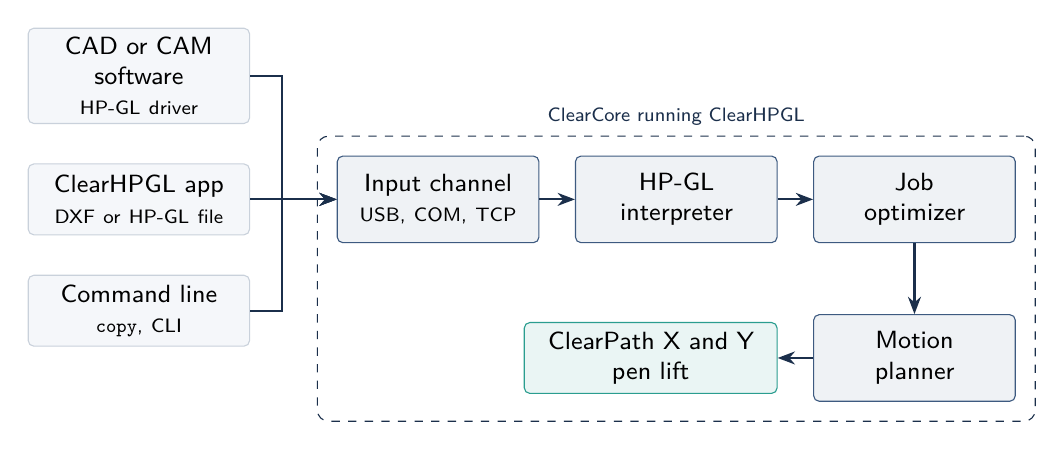
\begin{tikzpicture}[
  font=\sffamily\small,
  box/.style={draw=steel,fill=steel!8,rounded corners=2pt,align=center,
              minimum height=1.1cm,text width=2.35cm,inner sep=3pt},
  src/.style={draw=rulegray,fill=codebg,rounded corners=2pt,align=center,
              text width=2.6cm,minimum height=0.9cm,inner sep=3pt},
  outbox/.style={draw=teal,fill=teal!10,rounded corners=2pt,align=center,
              text width=2.6cm,minimum height=0.9cm,inner sep=3pt},
  arr/.style={-{Stealth[length=2.2mm]},thick,color=navy}]
  \node[src] (cad) {CAD or CAM software\\\scriptsize HP-GL driver};
  \node[src,below=0.5cm of cad] (app) {ClearHPGL app\\\scriptsize DXF or HP-GL file};
  \node[src,below=0.5cm of app] (cli) {Command line\\\scriptsize \texttt{copy}, CLI};
  \node[box,right=1.1cm of app] (ch) {Input channel\\\scriptsize USB, COM, TCP};
  \node[box,right=0.45cm of ch] (int) {HP-GL\\interpreter};
  \node[box,right=0.45cm of int] (opt) {Job\\optimizer};
  \node[box,below=0.9cm of opt] (mp) {Motion\\planner};
  \node[outbox,left=0.45cm of mp,text width=3.0cm] (mot) {ClearPath X and Y\\pen lift};
  \begin{scope}[on background layer]
    \node[draw=navy,dashed,rounded corners=4pt,inner sep=7pt,
          fit=(ch)(int)(opt)(mp),label={[font=\sffamily\scriptsize\color{navy}]north:ClearCore running ClearHPGL}] {};
  \end{scope}
  \draw[arr] (cad.east) -- ++(0.4,0) |- (ch.west);
  \draw[arr] (app.east) -- (ch.west);
  \draw[arr] (cli.east) -- ++(0.4,0) |- (ch.west);
  \draw[arr] (ch) -- (int);
  \draw[arr] (int) -- (opt);
  \draw[arr] (opt) -- (mp);
  \draw[arr] (mp) -- (mot);
\end{tikzpicture}
\caption{The path of a job through ClearHPGL}\label{fig:pipeline}
\end{figure}

\begin{description}[style=nextline,leftmargin=1.2em,font=\sffamily\bfseries\color{navy}]
  \item[Input channel] Receives jobs from all links. One source plots at a
        time, and the other sources wait. The channel does the flow control
        of a plotter (XON/XOFF and ENQ/ACK) and answers the \code{ESC .}
        device-control sequences. It removes the PCL and PJL wrappers that
        Windows drivers add.
  \item[HP-GL interpreter] Changes HP-GL into geometry, as an HP plotter
        does: scaling, rotation, clip windows, arcs and circles, and HP-GL/2
        encoded polylines. It gives a model name that you can set, so 7475A
        drivers and DraftMaster drivers both operate.
  \item[Job optimizer] For jobs from CAD software, keeps the full job and
        then plots it in a better order. Section~\ref{sec:optimizer} tells
        you more.
  \item[Motion planner] Moves the two servos as one coordinated machine,
        with lookahead and limits for acceleration and for speed at corners.
  \item[Safety] Monitors the emergency stop, the servo alerts, and the servo
        ready signals (HLFB) all the time. A fault disables the motors, stops
        the job, and latches until you clear it.
\end{description}

\section{What ClearHPGL Does Not Do}\label{sec:limits}

Table~\ref{tab:limits} shows the functions that this version does not have.
Do not plan a machine that needs them.

\begin{table}[htbp]
\centering
\caption{Functions not in firmware version 0.1.0}\label{tab:limits}
\begin{tabularx}{\linewidth}{@{}P{0.3\linewidth}L@{}}
\toprule
\textbf{Function} & \textbf{Result} \\
\midrule
Text (\cmd{LB}) & The board reads the text and does not draw it. The
\code{labels_skipped} counter in \cmd{status} shows how many labels it skipped.
Set your CAD software to send text as lines (``explode'' the text). \\
Area fills & \cmd{RA}, \cmd{RR}, and \cmd{WG} draw only the outline. \\
Line types and pen widths & All lines are solid. \cmd{LT} and \cmd{PW} have no effect. \\
Homing and limit switches & The machine has no home position. Plotter 0,0 is
where the pen is at power-up, or where you set the origin. \\
Pen changes & The machine has one pen. \cmd{SP} with a number above 1 does not
stop for a pen change. \\
Drag knives & The board does not offset the path for a tangential or drag knife. \\
Lasers & Laser control is a plan for the future. Chapter~\ref{ch:safety} tells
you why you must not connect a laser now. \\
\bottomrule
\end{tabularx}
\end{table}

\chapter{Safety}\label{ch:safety}

Read this chapter before you connect power to the machine. The servos of a
plotter are strong and fast. They can cause injury when they move.

\section{Status of the Software}

\begin{warning}
ClearHPGL is experimental. It is not certified for production or for
applications where safety is critical. Do not use it as the only safety
function of a machine. Install a physical emergency stop that removes power
from the motors.
\end{warning}

The emergency stop input of the board (\conn{DI-6}) stops the job and
disables the motors through the firmware. Firmware can fail. A hardware
emergency stop in the motor power circuit does not depend on the firmware.
You must have both.

\section{Motion That You Do Not Expect}

\begin{warning}
The motors enable automatically when a job arrives (setting
\key{auto_enable}~1). A job from a computer on the network can start the
machine at any time. Keep your hands and tools out of the work area when the
board has power and a computer is connected.
\end{warning}

\begin{warning}
Without limit switches, the machine has no protection at the ends of its
travel. It goes to the coordinates that the job gives, inside the plot area
that you set. If the plot area is larger than the mechanics, the carriage can
hit the end stops. Set \key{width_mm} and \key{height_mm} to the travel that
is really available. Limit switches (chapter~\ref{ch:limits}) stop the axis
with a ramp: they are not an emergency stop.
\end{warning}

\begin{itemize}
  \item Before you plot, look at the preview in the desktop app. Make sure
        that the drawing is in the plot area.
  \item Before you change the steps per revolution, the travel per
        revolution, or the direction of an axis, do a test move at low
        speed. Chapter~\ref{ch:setup} gives the procedure.
  \item Keep the work area clear of persons who do not operate the machine.
\end{itemize}

\section{Faults and the Emergency Stop}\label{sec:fault-behavior}

The board stops the machine when one of these conditions occurs:

\begin{itemize}
  \item The emergency stop input \conn{DI-6} opens (with the default setting
        \key{estop_di6}~1).
  \item A ClearPath servo reports an alert or a fault.
  \item The ready signal (HLFB) of a servo is not present when the motors
        enable (with \key{hlfb_check}~1).
\end{itemize}

When a fault occurs, the board disables the motors, drops the remainder of
the job, and latches the fault. The servos stop without control of
deceleration. The pen can stay on the material. To continue, remove the
cause, then clear the fault with the \cmd{clear} command or with
\menu{Clear fault} in the desktop app.

\begin{caution}
When the motors disable, the axes are free. On a vertical machine or a
machine on a slope, gravity can move an axis. Make sure that the axes cannot
fall or move when the motors have no power.
\end{caution}

\begin{note}
\notelabel If you do not connect an emergency stop to \conn{DI-6}, set
\key{estop_di6} to 0. If you do not do this, the board stays in the fault
state and does not plot. A hardware emergency stop in the motor power circuit
is still necessary.
\end{note}

\section{Lasers}

\begin{warning}
Do not connect a laser to the pen output. The pen output turns on and off
with the timing of a pen: it has settle delays and no control of power. The
firmware has no interlocks for an enclosure, a lid, or air assist. A laser on
this output can cause fire, burns, and damage to the eyes.
\end{warning}

Laser control is a plan for a future version. It will need control of the
power by the speed of the path, and interlocks that can stop the beam.

\section{Electrical Safety}

\begin{warning}
Disconnect all power before you connect or disconnect the motors, the pen
lift, or the emergency stop. The ClearPath servos and their power supplies
have dangerous voltages. Obey the instructions of Teknic for the hardware.
\end{warning}

\begin{caution}
The board writes its settings to nonvolatile memory. It can do this only
when the supply voltage is above the undervoltage limit of the ClearCore. Do
not change settings while the ClearCore gets its power only from the USB
cable.
\end{caution}

\chapter{Hardware and Connections}\label{ch:hardware}

\section{Parts}

Table~\ref{tab:parts} lists the parts of a ClearHPGL plotter. The mechanics
(the frame, the guides, and the belts or screws) are your design. The
firmware drives two axes and a pen lift, so the plot area is the travel that
your mechanics give.

\begin{table}[htbp]
\centering
\caption{Parts of a ClearHPGL plotter}\label{tab:parts}
\begin{tabularx}{\linewidth}{@{}P{0.3\linewidth}L@{}}
\toprule
\textbf{Part} & \textbf{Function and notes} \\
\midrule
Teknic ClearCore & Runs the firmware. Needs its own 24~V DC supply. \\
Two ClearPath-SD servos & Step-and-direction servos for X and Y. Each one
needs its HLFB (ready) output connected. \\
Pen lift & A solenoid or a relay on a digital output, or a third ClearPath
servo on \conn{M2}. \\
Emergency stop & A normally closed contact on \conn{DI-6}, and a separate
contact that removes power from the motors. \\
Network cable or USB cable & The link to the computer. A serial cable on
\conn{COM-0} or \conn{COM-1} is also possible. \\
Windows computer & For the desktop app and the CAD software. The app is
optional. \\
\bottomrule
\end{tabularx}
\end{table}

\section{Connector Map}

Table~\ref{tab:connectors} shows what each connector of the ClearCore does
with the default settings.

\begin{table}[htbp]
\centering
\caption{ClearCore connectors used by ClearHPGL}\label{tab:connectors}
\begin{tabularx}{\linewidth}{@{}P{0.16\linewidth}P{0.28\linewidth}L@{}}
\toprule
\textbf{Connector} & \textbf{Function} & \textbf{Setting} \\
\midrule
\conn{M0} & X axis (CoreXY: motor A), ClearPath, step and direction & \key{steps_rev_x}, \key{mm_rev_x}, \key{dir_x}, \key{kinematics} \\
\conn{M1} & Y axis (CoreXY: motor B), ClearPath, step and direction & \key{steps_rev_y}, \key{mm_rev_y}, \key{dir_y}, \key{swap_xy} \\
\conn{M2} & Pen lift servo (optional) & \key{pen_mode}~1 and the \key{z_*} settings \\
\conn{IO-0} & Pen lift output (default) & \key{pen_mode}~0, \key{pen_io}, \key{pen_active_high} \\
\conn{DI-6} & Emergency stop input & \key{estop_di6} \\
\conn{COM-0}, \conn{COM-1} & HP-GL serial port (off by default) & \key{com_port}, \key{com_baud}, \key{com_handshake}, \key{com_rs232} \\
USB & HP-GL and the setup console & none \\
Ethernet & HP-GL (TCP 9100), console (TCP 9300), discovery (UDP 9302) & \key{net_mode}, \key{ip}, \key{netmask}, \key{gateway} \\
\bottomrule
\end{tabularx}
\end{table}

\begin{figure}[htbp]
\centering
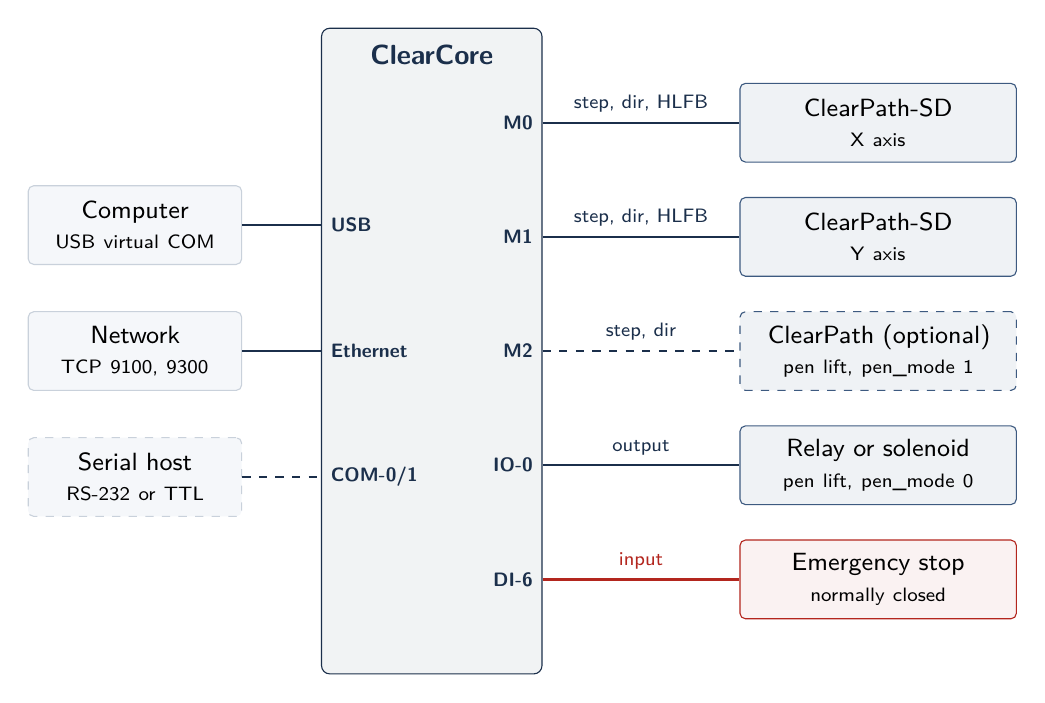
\begin{tikzpicture}[font=\sffamily\small,
  cc/.style={draw=navy,fill=navy!6,rounded corners=3pt,minimum width=2.8cm,minimum height=8.2cm},
  dev/.style={draw=steel,fill=steel!8,rounded corners=2pt,align=center,text width=3.3cm,minimum height=1.0cm,inner sep=3pt},
  pc/.style={draw=rulegray,fill=codebg,rounded corners=2pt,align=center,text width=2.5cm,minimum height=1.0cm,inner sep=3pt},
  conpin/.style={font=\sffamily\scriptsize\bfseries,color=navy},
  w/.style={thick,color=navy},
  ws/.style={thick,color=signal}]
  \node[cc] (cc) {};
  \node[font=\sffamily\bfseries\color{navy}] at ([yshift=-0.35cm]cc.north) {ClearCore};
  % right side: motion
  \node[conpin,anchor=east] (m0) at ([yshift=2.9cm]cc.east) {M0};
  \node[conpin,anchor=east] (m1) at ([yshift=1.45cm]cc.east) {M1};
  \node[conpin,anchor=east] (m2) at ([yshift=0.0cm]cc.east) {M2};
  \node[conpin,anchor=east] (io0) at ([yshift=-1.45cm]cc.east) {IO-0};
  \node[conpin,anchor=east] (di6) at ([yshift=-2.9cm]cc.east) {DI-6};
  \node[dev,anchor=west] (x) at ([xshift=2.5cm]m0.east) {ClearPath-SD\\\scriptsize X axis};
  \node[dev,anchor=west] (y) at ([xshift=2.5cm]m1.east) {ClearPath-SD\\\scriptsize Y axis};
  \node[dev,anchor=west,dashed] (z) at ([xshift=2.5cm]m2.east) {ClearPath (optional)\\\scriptsize pen lift, pen\_mode 1};
  \node[dev,anchor=west] (pen) at ([xshift=2.5cm]io0.east) {Relay or solenoid\\\scriptsize pen lift, pen\_mode 0};
  \node[dev,anchor=west,draw=signal,fill=signal!6] (es) at ([xshift=2.5cm]di6.east) {Emergency stop\\\scriptsize normally closed};
  \draw[w] (m0.east) -- node[above,font=\sffamily\scriptsize]{step, dir, HLFB} (x.west);
  \draw[w] (m1.east) -- node[above,font=\sffamily\scriptsize]{step, dir, HLFB} (y.west);
  \draw[w,dashed] (m2.east) -- node[above,font=\sffamily\scriptsize]{step, dir} (z.west);
  \draw[w] (io0.east) -- node[above,font=\sffamily\scriptsize]{output} (pen.west);
  \draw[ws] (di6.east) -- node[above,font=\sffamily\scriptsize]{input} (es.west);
  % left side: links
  \node[conpin,anchor=west] (usb) at ([yshift=1.6cm]cc.west) {USB};
  \node[conpin,anchor=west] (eth) at ([yshift=0.0cm]cc.west) {Ethernet};
  \node[conpin,anchor=west] (com) at ([yshift=-1.6cm]cc.west) {COM-0/1};
  \node[pc,anchor=east] (pcu) at ([xshift=-1.0cm]usb.west) {Computer\\\scriptsize USB virtual COM};
  \node[pc,anchor=east] (pce) at ([xshift=-1.0cm]eth.west) {Network\\\scriptsize TCP 9100, 9300};
  \node[pc,anchor=east,dashed] (pcc) at ([xshift=-1.0cm]com.west) {Serial host\\\scriptsize RS-232 or TTL};
  \draw[w] (pcu.east) -- (usb.west);
  \draw[w] (pce.east) -- (eth.west);
  \draw[w,dashed] (pcc.east) -- (com.west);
\end{tikzpicture}
\caption{Connections of a ClearHPGL plotter. Dashed parts are optional.}\label{fig:wiring}
\end{figure}

\section{ClearPath Servos}

Connect the X servo to \conn{M0} and the Y servo to \conn{M1}. Use the
ClearPath MSP software from Teknic to set each servo before you connect it.

\begin{procedure}{Prepare a ClearPath-SD servo}
\begin{enumerate}
  \item Connect the servo to the computer with its USB cable, and start
        ClearPath MSP.
  \item Set the input format to step and direction.
  \item Set the input resolution (the steps per revolution). Use the same
        value later in \key{steps_rev_x} or \key{steps_rev_y}. The default is 800.
  \item Set the HLFB output to a mode with a PWM output, with a carrier
        frequency of 482~Hz. The ClearCore examples from Teknic use
        ``ASG-Position w/Measured Torque.''
  \item Tune the servo for the load of its axis, as the ClearPath manual
        tells you.
  \item Save the configuration to the servo.
\end{enumerate}
\end{procedure}

The firmware reads the HLFB signal of each servo. When the motors enable,
the board waits for HLFB from all servos. If HLFB does not come, the board
disables the motors and reports a fault. Set \key{hlfb_check} to 0 only if
your servos do not supply HLFB.

\begin{note}
\notelabel Use the same steps per millimeter on X and Y. The planner uses the
scale of the X axis for the speed and the acceleration of the path. Arcs
operate as true arcs only when the two scales are the same.
\end{note}

\section{CoreXY and H-Bot Machines}\label{sec:corexy}

In a \term{CoreXY} or an H-bot machine, the two motors do not each drive one
axis. Two belts move the head together: when both motors turn the same
direction, the head moves in X; when they turn in opposite directions, it
moves in Y. One motor alone moves the head diagonally.

Set \key{kinematics} to 1 for these machines. The board then plans and draws
in X and Y as usual, and sends these step counts to the motors:

\begin{center}
\begin{tabular}{@{}lll@{}}
\toprule
\textbf{Connector} & \textbf{Motor} & \textbf{Steps} \\
\midrule
\conn{M0} & A & X + Y \\
\conn{M1} & B & X $-$ Y \\
\bottomrule
\end{tabular}
\end{center}

\begin{itemize}
  \item Both belts run on pulleys with the same pitch diameter. Set it in
        \key{pulley_dia_mm}. The travel of the belt for one revolution is
        $\pi$ multiplied by the pitch diameter; \key{mm_rev_x} and
        \key{mm_rev_y} are not used. The default, \SI{12.7324}{mm}, is a
        20-tooth GT2 pulley (\SI{40}{mm} per revolution).
  \item The pitch diameter is the number of teeth multiplied by the belt
        pitch, divided by $\pi$. For example, a 16-tooth GT2 pulley (2~mm
        pitch) has a pitch diameter of 32/$\pi$ = \SI{10.186}{mm}.
  \item Both motors must have the same steps per revolution. The board
        refuses \key{kinematics}~1 if \key{steps_rev_x} and \key{steps_rev_y}
        are different.
  \item On a 45° move, one motor does all the work. It turns 1.41 times faster
        than the head moves, and accelerates 1.41 times faster. Set
        \key{motor_max_mm_s} to the highest belt speed that your motors can
        hold. The board then decreases the speed of each segment that would
        make a motor go faster.
  \item \key{corner_mm_s} limits the change of speed of each motor at a corner.
\end{itemize}

The direction of each motor and the sequence of the belts change how the
head moves. The settings \key{dir_x}, \key{dir_y}, and \key{swap_xy}
(exchange X and Y) correct all the possible layouts. You do not have to
change the wiring. Section~\ref{sec:corexy-check} gives the procedure.

\section{Pen Lift}

The firmware has two types of pen lift. Select one with \key{pen_mode}.

\subsection{Digital Output (\key{pen_mode}~0)}

The default. A digital output (\conn{IO-0} by default) operates a relay or a
solenoid. With \key{pen_active_high}~1, the output is on when the pen is
down. After the board lowers or raises the pen, it waits for the settle time
(\key{pen_down_ms}, default 150~ms; \key{pen_up_ms}, default 100~ms) before
the axes move.

\begin{caution}
Examine the current rating of the ClearCore output in the ClearCore manual.
If the solenoid needs more current, use a relay. Install a flyback diode
across a coil that has no internal diode.
\end{caution}

\subsection{Servo on M2 (\key{pen_mode}~1)}

A third ClearPath servo on \conn{M2} moves the pen to two positions:
\key{z_up_steps} (default 0) and \key{z_down_steps} (default 800). Its speed
and acceleration are \key{z_vel_steps} and \key{z_accel_steps}.

\begin{caution}
The M2 servo has no home position. Before you supply power, put the pen at
the pen-up position. The board uses the position at power-up as step 0.
\end{caution}

\section{Emergency Stop}

Connect a normally closed emergency stop contact to \conn{DI-6}. With the
default \key{estop_di6}~1, the board sees a fault when the input is low
(the contact is open, or a wire is broken). Table~\ref{tab:estop} shows the
three values.

\begin{table}[htbp]
\centering
\caption{Values of \key{estop_di6}}\label{tab:estop}
\begin{tabularx}{\linewidth}{@{}P{0.12\linewidth}L@{}}
\toprule
\textbf{Value} & \textbf{Result} \\
\midrule
0 & The board does not monitor \conn{DI-6}. Use only if no emergency stop is connected. \\
1 & Fault when \conn{DI-6} is low. Use with a normally closed contact (default). \\
2 & Fault when \conn{DI-6} is high. Use with a normally open contact. \\
\bottomrule
\end{tabularx}
\end{table}

\section{Links to the Computer}

\begin{description}[style=nextline,leftmargin=1.2em,font=\sffamily\bfseries\color{navy}]
  \item[USB] The board shows as a virtual COM port. It receives HP-GL at any
        baud rate. Type \cmd{menu} on a line by itself to open the setup
        console.
  \item[Ethernet] The board uses DHCP by default. If DHCP fails, the address is
        192.168.0.110. It receives HP-GL on TCP port 9100 and gives the
        console on TCP port 9300.
  \item[COM-0 or COM-1] An RS-232 or TTL serial port for HP-GL. It is off by
        default. Set \key{com_port}, \key{com_baud}, \key{com_handshake}, and
        \key{com_rs232}, then restart the board.
\end{description}

\chapter{Install the Firmware}\label{ch:firmware}

This chapter tells you how to load the firmware into the ClearCore. The
easiest way is from the desktop app (section~\ref{sec:fw-app}). To build the
firmware from its source, use the procedure in
section~\ref{sec:fw-build}.

\section{What You Need}

\begin{itemize}
  \item A USB cable from the computer to the ClearCore.
  \item A 24~V supply for the ClearCore. The board must not get its power
        only from USB when it writes its settings.
  \item From the app: the ClearHPGL desktop app. It carries the firmware and
        the flash tool in its \file{firmware} directory.
  \item To build from the source: a Windows computer with Microchip Studio 7
        (formerly Atmel Studio 7) and the ClearHPGL source repository. The
        build script uses the ARM compiler and the \file{make.exe} of
        Microchip Studio. The repository contains the flash tools:
        \file{tools/bossac/bossac.exe} and \file{tools/flash_clearcore.cmd},
        from Teknic.
\end{itemize}

\section{Update from the App}\label{sec:fw-app}

The desktop app carries the firmware that it was built with. It can put that
firmware on the ClearCore over USB. You do not need Microchip Studio or a
command line.

\begin{warning}
Updating restarts the board. Make sure that no job is plotting and that the
work area is clear. If the motors are enabled, the update disables them
first.
\end{warning}

\begin{procedure}{Update the firmware from the app}
\begin{enumerate}
  \item Connect the ClearCore to the computer with the USB cable.
  \item In the app, select \menu{Plotter\,>\,Update board firmware\ldots}. If
        the app is connected to the board over USB, it disconnects first.
  \item In \menu{USB port}, select the ClearCore. The window shows the
        firmware on the board and the firmware that the app carries
        (figure~\ref{fig:fwdialog}).
  \item Click \menu{Update to} (or \menu{Reinstall}) and wait. Do not
        disconnect the cable.
  \item Make sure that the window shows ``Firmware \ldots\ is running.''
  \item Click \menu{Close}. The app connects to the board again.
\end{enumerate}
\end{procedure}

\begin{figure}[htbp]
\centering
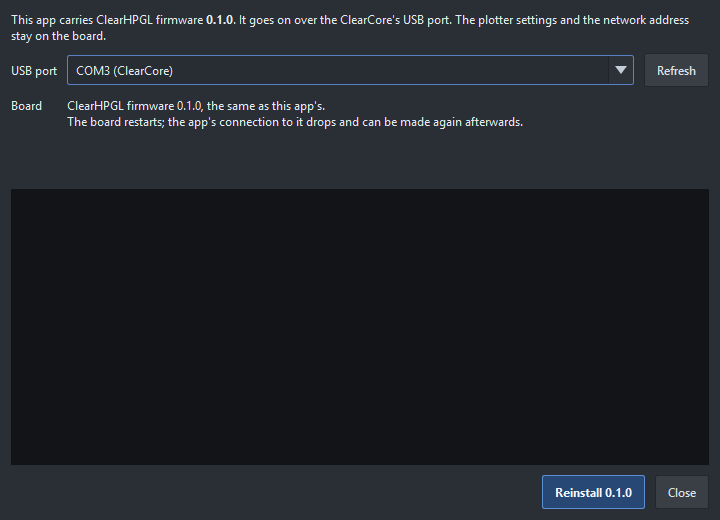
\includegraphics[width=0.8\linewidth]{firmware-dialog.png}
\caption{\menu{Update board firmware}, with the board read on COM3}\label{fig:fwdialog}
\end{figure}

The update keeps all settings of the board: the plot area, the speeds, and
the network address. They are in a part of the memory that the update does
not erase. The update does not start while a job plots.

\section{Flash Without the App}\label{sec:fw-cmd}

The installer also puts a flash tool in the \file{firmware} directory of the
app. Use it if the app cannot run.

\begin{procedure}{Flash the firmware from the Start menu}
\begin{enumerate}
  \item Connect the ClearCore to the computer with the USB cable.
  \item Close the ClearHPGL app. It can hold the USB port.
  \item Select \menu{ClearHPGL\,>\,Flash the ClearCore firmware (USB)} in the
        Start menu.
  \item Wait until the window shows \code{Success!}, then press a key.
\end{enumerate}
\end{procedure}

This also keeps the settings of the board.

\begin{note}
\notelabel If the update stops (for example, the cable is disconnected), the
board can have no firmware. Push the reset button of the ClearCore two times
quickly, so that the IO-0 to IO-5 lights move in sequence. Then click
\menu{Refresh} and update again.
\end{note}

\section{Build and Load the Firmware}\label{sec:fw-build}

\begin{warning}
Loading firmware restarts the board. Make sure that no job is plotting and
that the work area is clear before you start.
\end{warning}

\begin{procedure}{Build the firmware and load it into the ClearCore}
\begin{enumerate}
  \item Connect the ClearCore to the computer with the USB cable.
  \item Close all programs that use the USB COM port of the board: a serial
        terminal, the desktop app, or a CAD plotter driver.
  \item Open PowerShell in the root directory of the repository.
  \item Type this command and press Enter:
\begin{lstlisting}[language=console]
./Firmware/build.ps1 -Flash
\end{lstlisting}
  \item Wait. The script builds LwIP, libClearCore, and the firmware. Then it
        finds the board, puts it into its bootloader, and writes the
        firmware.
  \item Make sure that the output contains the line \code{Verify successful}.
\end{enumerate}
\end{procedure}

Without \code{-Flash}, the script only builds. The firmware files are in
\file{Firmware/ClearCoreFirmware/Release/}: \file{ClearHPGL_Firmware.bin} and
\file{ClearHPGL_Firmware.uf2}. To load a \file{.bin} file that you received
from a different person, use this command:

\begin{lstlisting}[language=console]
tools\flash_clearcore.cmd path\to\ClearHPGL_Firmware.bin
\end{lstlisting}

\begin{note}
\notelabel The flash script looks for the board on its normal USB port. Then
it waits for the bootloader port. The two ports have different COM numbers.
This is correct. If the script cannot find the board, push the reset button
of the ClearCore two times quickly to start the bootloader, then run the
script again.
\end{note}

\section{Make Sure That the Firmware Operates}

\begin{procedure}{Examine the firmware after you load it}
\begin{enumerate}
  \item Open the USB COM port of the board in a serial terminal (for example
        PuTTY). The baud rate has no effect.
  \item Type \cmd{menu} on a line by itself and press Enter. The console
        shows its list of commands.
  \item Type \cmd{version} and press Enter. Make sure that the version is the
        one that you loaded.
  \item Type \cmd{status} and press Enter. Make sure that \code{fault=none}.
  \item Type \cmd{exit} and press Enter to close the console.
\end{enumerate}
\end{procedure}

The settings stay in the board when you load new firmware. A new firmware
version that adds a setting gives it its default value.

\section{Settings of Other Firmware}

The settings of ClearHPGL have their own marker (\code{CHPG}) in the
nonvolatile memory. If the board ran ClearCoreROS or ClearAI before, and
ClearHPGL has no saved settings yet, ClearHPGL keeps the network settings of
that firmware, so the board keeps its IP address. All other settings start at
their defaults.

\chapter{First Setup}\label{ch:setup}

Do the procedures in this chapter in the given sequence when you start a new
machine. You can do them in the console of the board, or in
\menu{Plotter settings} in the desktop app (section~\ref{sec:app-settings}).

\section{Open the Console}\label{sec:console}

The console is a text interface for setup and for diagnosis. It is available
on two links:

\begin{description}[style=nextline,leftmargin=1.2em,font=\sffamily\bfseries\color{navy}]
  \item[USB] Open the USB COM port in a serial terminal. Type \cmd{menu} on a
        line by itself and press Enter. Type \cmd{exit} to go back to HP-GL
        mode. While the console is open, the USB port does not receive HP-GL.
  \item[TCP port 9300] Connect a terminal (for example PuTTY in ``raw'' mode,
        or \code{ncat}) to port 9300 of the board. The console accepts one
        client at a time. The desktop app uses this port when it is connected
        over Ethernet.
\end{description}

Each command ends with a line that starts with \code{ok} or \code{error:}.
Appendix~\ref{app:console} lists all commands. These are the commands that
you use most:

\begin{lstlisting}[language=console]
status                 # state, position, pen, counters, and links
config                 # all settings and their values
set <key> <value>      # change a setting and save it
enable / disable       # supply or remove motor power
goto <x_mm> <y_mm>     # pen-up move to a position
pen up / pen down      # test the pen lift
origin                 # the present position becomes plotter 0,0
clear                  # clear a latched fault
\end{lstlisting}

\subsection{When a Setting Takes Effect}

Each setting has a rule for when you can change it. The \cmd{config} command
shows the rule at the end of the line. The desktop app shows it as a label
next to the field.

\begin{table}[htbp]
\centering
\caption{When a setting can change}\label{tab:when}
\begin{tabularx}{\linewidth}{@{}P{0.17\linewidth}P{0.2\linewidth}L@{}}
\toprule
\textbf{Mark in \cmd{config}} & \textbf{Label in the app} & \textbf{Rule} \\
\midrule
(none) & (none) & Live. The change takes effect immediately, also during a job. \\
\code{[idle]} & between jobs & The board refuses the change while a job plots. The motors can stay enabled. \\
\code{[disabled]} & motors disabled & The board refuses the change while the motors are enabled. Use \cmd{disable} first. The app does this for you. \\
\code{[restart]} & after restart & The board saves the change. It takes effect after \cmd{restart}. \\
\bottomrule
\end{tabularx}
\end{table}

\section{Set the Kinematics}

Set the kinematics first. It is the first setting in \cmd{config} and in the
app, because it selects the mechanics settings that apply.

\begin{itemize}
  \item \key{kinematics}~0, Cartesian (default): one motor for each axis.
        \conn{M0} moves X and \conn{M1} moves Y.
  \item \key{kinematics}~1, CoreXY or H-bot: two belts move the head together
        (section~\ref{sec:corexy}).
\end{itemize}

\begin{procedure}{Set the kinematics}
\begin{enumerate}
  \item Type \cmd{disable}.
  \item Type \cmd{set kinematics 0} for a Cartesian machine, or
        \cmd{set kinematics 1} for a CoreXY or H-bot machine. The present
        position becomes the origin.
\end{enumerate}
\end{procedure}

\section{Set the Mechanics}

The board must know how far the head moves for one revolution of a motor.

\begin{itemize}
  \item \key{steps_rev_x}, \key{steps_rev_y}: the steps per revolution of
        \conn{M0} and \conn{M1}. Use the input resolution that you set in
        ClearPath MSP. Default 800.
  \item Cartesian: \key{mm_rev_x}, \key{mm_rev_y}: the travel of the axis for
        one revolution of the motor, in mm. Default 5.0. For a lead screw, it
        is the lead of the screw. For a belt, it is the number of pulley teeth
        multiplied by the belt pitch.
  \item CoreXY: \key{pulley_dia_mm}: the pitch diameter of the pulleys, in
        mm, for both motors. Default \SI{12.7324}{mm} (a 20-tooth GT2 pulley).
        The pitch diameter is the number of teeth multiplied by the belt
        pitch, divided by $\pi$.
\end{itemize}

\begin{procedure}{Set the mechanics of a CoreXY machine}
\begin{enumerate}
  \item Type \cmd{disable}.
  \item Type \cmd{set steps_rev_x 800} and \cmd{set steps_rev_y 800}. Use the
        value from ClearPath MSP. The two values must be the same.
  \item Type \cmd{set pulley_dia_mm 12.7324}. Use the pitch diameter of your
        pulleys.
  \item Type \cmd{config}, and make sure that the values are correct.
\end{enumerate}
\end{procedure}

\begin{procedure}{Set the steps and the travel per revolution (Cartesian)}
\begin{enumerate}
  \item Type \cmd{disable}.
  \item Type \cmd{set steps_rev_x 800}. Use the value from ClearPath MSP.
  \item Type \cmd{set mm_rev_x 40}. Use the travel of your X axis.
  \item Do steps 2 and 3 again for Y, with \key{steps_rev_y} and \key{mm_rev_y}.
  \item Type \cmd{config}, and make sure that the four values are correct.
\end{enumerate}
\end{procedure}

\begin{note}
\notelabel On a Cartesian machine, use the same steps per millimeter on X and
Y. If the two axes are different, the speeds use the X scale, and arcs are
drawn as short straight lines. On a CoreXY machine, the scales are always the
same.
\end{note}

\section{Set the Plot Area and the Origin}

The \term{plot area} is \key{width_mm} by \key{height_mm} (default
400 by 300). It is the \term{hard clip}: the board does not draw outside it.
Plotter 0,0 is the lower-left corner of the plot area. The position of the
pen at power-up is 0,0, until you set a different origin.

\begin{warning}
The board does not know where the end stops of your machine are. Set the plot
area to the travel that is really available from the origin. If the area is
too large, the carriage can hit the end of its travel.
\end{warning}

\begin{procedure}{Set the plot area and the origin}
\begin{enumerate}
  \item Measure the travel of each axis from the corner that you want as the
        origin.
  \item Type \cmd{set width_mm 600}. Use your X travel.
  \item Type \cmd{set height_mm 300}. Use your Y travel.
  \item Move the pen to the lower-left corner of the plot area. Use
        \cmd{goto} or the \menu{Jog} tab of the app.
  \item Type \cmd{origin}. The present position becomes plotter 0,0.
\end{enumerate}
\end{procedure}

\begin{note}
\notelabel The board does not keep the origin when it restarts. After power-up,
the origin is where the pen is. Move the pen to the corner before you supply
power, or set the origin again.
\end{note}

\section{Make Sure That the Axes Move Correctly}

\begin{warning}
Keep your hands out of the work area. The axes move when you send the next
commands.
\end{warning}

\begin{procedure}{Do the first moves}
\begin{enumerate}
  \item Type \cmd{set draw_mm_s 20} and \cmd{set travel_mm_s 20} to get a low speed.
  \item Type \cmd{enable}. Make sure that the reply is \code{ok}.
  \item Type \cmd{goto 50 0}. The pen must move \SI{50}{mm} in the positive
        X direction (to the right on a standard plotter).
  \item Measure the distance. If it is not \SI{50}{mm}, examine
        \key{steps_rev_x} and \key{mm_rev_x}.
  \item If the axis moved in the wrong direction, type \cmd{goto 0 0},
        \cmd{disable}, then \cmd{set dir_x -1}.
  \item Do steps 3 to 5 again for Y with \cmd{goto 0 50} and \key{dir_y}.
  \item Type \cmd{goto 0 0} to go back to the origin.
\end{enumerate}
\end{procedure}

\subsection{CoreXY and H-Bot Machines}\label{sec:corexy-check}

On a CoreXY or an H-bot machine (section~\ref{sec:corexy}), set the
kinematics first. Then find the correct directions with this procedure.

\begin{warning}
With the wrong kinematics or directions, the head can move in a direction
that you do not expect. Use a low speed and short moves, and keep the head
away from the ends of its travel.
\end{warning}

\begin{procedure}{Set the kinematics and the directions of a CoreXY machine}
\begin{enumerate}
  \item Type \cmd{disable}.
  \item Make sure that \key{kinematics} is 1 and that the steps per
        revolution and \key{pulley_dia_mm} are set.
  \item Type \cmd{set draw_mm_s 20} and \cmd{set travel_mm_s 20}.
  \item Type \cmd{enable}, then \cmd{goto 20 0}.
  \item Look at the movement of the head, and find it in
        table~\ref{tab:corexy-fix}.
  \item Type \cmd{disable}, then do the correction in the table.
  \item Type \cmd{origin}, and do steps 4 to 6 again until the head moves
        \SI{20}{mm} to the right.
  \item Type \cmd{goto 20 20}. The head must move \SI{20}{mm} up (positive Y).
        If it moves down, type \cmd{disable}, set \key{dir_y} to the other
        value, type \cmd{origin}, and do this step again from \cmd{goto 20 0}.
\end{enumerate}
\end{procedure}

\begin{table}[htbp]
\centering
\caption{Corrections for a CoreXY machine after \cmd{goto 20 0}}\label{tab:corexy-fix}
\begin{tabularx}{\linewidth}{@{}P{0.38\linewidth}L@{}}
\toprule
\textbf{The head moves} & \textbf{Correction} \\
\midrule
Right (positive X) & Correct. Go to the last step. \\
Left (negative X) & Set \key{dir_x} to the other value (1 or -1). \\
Up or down (Y) & Set \key{swap_xy} to the other value (0 or 1). \\
Diagonally & \key{kinematics} is not 1, or the belts are not a CoreXY or H-bot layout. \\
\bottomrule
\end{tabularx}
\end{table}

\section{Set the Pen Lift}

\begin{procedure}{Set and test the pen lift}
\begin{enumerate}
  \item Type \cmd{disable}.
  \item Type \cmd{set pen_mode 0} for a digital output, or \cmd{set pen_mode 1}
        for a servo on \conn{M2}.
  \item For a digital output, set \key{pen_io} (0 to 5) and \key{pen_active_high}.
  \item For a servo on \conn{M2}, set \key{z_up_steps} and \key{z_down_steps}.
  \item Type \cmd{enable}.
  \item Type \cmd{pen down}. Make sure that the pen goes down.
  \item Type \cmd{pen up}. Make sure that the pen goes up.
  \item If the pen moves before it is fully down or up, increase
        \key{pen_down_ms} or \key{pen_up_ms}.
\end{enumerate}
\end{procedure}

\section{Set the Speeds}

Table~\ref{tab:speeds} shows the motion settings. All of them are live, so
you can change them during a test plot and see the result.

\begin{table}[htbp]
\centering
\caption{Motion settings}\label{tab:speeds}
\begin{tabularx}{\linewidth}{@{}P{0.21\linewidth}P{0.15\linewidth}L@{}}
\toprule
\textbf{Setting} & \textbf{Default} & \textbf{Function} \\
\midrule
\key{draw_mm_s} & 100 mm/s & Speed with the pen down. \\
\key{travel_mm_s} & 200 mm/s & Speed with the pen up. \\
\key{max_mm_s} & 250 mm/s & Highest pen-down speed that a job can ask for with \cmd{VS}. \\
\key{job_speed} & 1 & 1: the speed in the job (\cmd{VS}) sets the pen-down speed. 0: always use \key{draw_mm_s}. \\
\key{accel_mm_s2} & 2000 mm/s\textsuperscript{2} & Acceleration along the path. It also limits the speed on curves. \\
\key{corner_mm_s} & 20 mm/s & Largest change of speed of one motor at a corner. A larger value gives faster corners and more shock to the machine. \\
\key{motor_max_mm_s} & 0 (none) & Highest speed of a motor, as belt travel. For CoreXY, where a motor can turn 1.41 times faster than the head moves. \\
\bottomrule
\end{tabularx}
\end{table}

Start with low values. Increase them until the machine is fast and the lines
are still clean. A heavy carriage or a long belt needs a lower acceleration.

\section{Set the Network}

The board uses DHCP by default. If it gets no address, it uses
192.168.0.110. For a fixed address, do this procedure.

\begin{procedure}{Set a static IP address}
\begin{enumerate}
  \item Type \cmd{set net_mode 1}.
  \item Type \cmd{set ip 10.168.41.5}. Use your address.
  \item Type \cmd{set netmask 255.255.255.0}.
  \item Type \cmd{set gateway 10.168.41.1}. If no other network must reach the
        board, you can keep 0.0.0.0.
  \item Type \cmd{restart}. The board restarts with the new address.
  \item From the computer, type \cmd{ping 10.168.41.5} to make sure that the
        board replies.
\end{enumerate}
\end{procedure}

To go back to DHCP, type \cmd{set net_mode 0} and \cmd{restart}.

\section{Do a Test Plot}

Send a small square to the board. On Windows, save this text in a file with
the name \file{square.plt}:

\begin{lstlisting}[language=hpgl]
IN;SP1;PU400,400;PD2400,400,2400,2400,400,2400,400,400;PU0,0;
\end{lstlisting}

This draws a \SI{50}{mm} square that starts \SI{10}{mm} from the origin.
Send it to the USB port (for example COM3) with this command in
\file{cmd.exe}:

\begin{lstlisting}[language=console]
copy /b square.plt COM3
\end{lstlisting}

The motors enable automatically, the square plots, and the pen goes back to
0,0. Measure the square. Each side must be \SI{50}{mm}.

\begin{note}
\notelabel The board keeps a job from the USB port until the port is quiet
for 2~s, and then plots it in a better order (section~\ref{sec:optimizer}).
Thus the plot starts approximately 2~s after the file is sent.
\end{note}

\chapter{Limits and Homing}\label{ch:limits}

Limit switches and homing are optional. Without them, the board does not know
where the ends of the axes are: the plot area and the origin are all that keep
the pen on the bed (section~\ref{sec:plot-area}). With them:

\begin{itemize}
  \item A \term{limit switch} stops the motion of an axis toward the end of
        its travel. A job that reaches a limit stops, and the board drops it.
  \item A \term{home switch} gives the axis a known position. After homing,
        plotter 0,0 is at the same place on the bed each time.
\end{itemize}

The switches belong to the axes as HP-GL sees them (X and Y), not to the
motors. Thus they operate the same way on a Cartesian machine, on a CoreXY
machine, and with \key{dir_x}, \key{dir_y}, or \key{swap_xy}.

\begin{warning}
A limit switch is not an emergency stop. The board stops the axis with a
ramp, so the axis moves past the switch before it stops. Connect an emergency
stop to \conn{DI-6} (section~\ref{sec:fault-behavior}) and keep space for the stop
distance after each limit switch.
\end{warning}

\section{How the Board Uses the Switches}\label{sec:switch-rules}

\paragraph{Inputs.} Each switch uses one input of the ClearCore:
\conn{DI-7}, \conn{DI-8}, \conn{A-9} to \conn{A-12}, or \conn{IO-0} to
\conn{IO-5}. The board does not let two switches use the same input, with one
exception: the home switch of an axis can use the input of a limit switch of
the same axis. Then the axis homes on that limit switch. \conn{DI-6} is for the
emergency stop, and the pen output (\key{pen_io}) cannot be a switch.

\paragraph{Contacts.} A \term{normally closed} switch is on at rest and off
when it trips. This is the default and the recommended contact: a broken wire
reads as a tripped switch, so the axis stops. A \term{normally open} switch is
off at rest. Set its bit in \key{switch_open} (table~\ref{tab:set-switches}).

\paragraph{Filter.} The board reads the inputs at 5~kHz, in the same interrupt
that makes the steps. A switch changes state when its input has the new level
for three samples in a row (0.6~ms). The board keeps the position of the first
of the three samples. This is the position where the switch tripped.

\paragraph{Limits.} A tripped limit switch stops only the motion
\emph{toward} it. Motion away from it is always possible, so you can move the
axis off the switch. The stop is a ramp along the path at three times
\key{accel_mm_s2}. It starts in the same sample in which the switch trips. The
distance after the switch is approximately:
\begin{equation}
  d = \frac{v^{2}}{2 \times 3 \times a} + v \times 0.6\ \text{ms}
\end{equation}
where $v$ is the speed and $a$ is \key{accel_mm_s2}. For example, at
200~mm/s and 2000~mm/s\textsuperscript{2}, $d \approx 3.5$~mm. At a jog speed
of 10~mm/s, $d$ is less than 0.02~mm.

\begin{table}[htbp]
\centering
\caption{What a limit switch does}\label{tab:limit-actions}
\begin{tabularx}{\linewidth}{@{}P{0.28\linewidth}L@{}}
\toprule
\textbf{Motion} & \textbf{Result} \\
\midrule
A job, \cmd{goto}, or \cmd{pen} & The axis stops. The board drops the job and
raises the pen. The fault \code{limit X+ (DI-7)} (for example) latches. The
motors stay enabled. The next job waits until you type \cmd{clear}. \\
A jog & The jog stops. This is not a fault. A jog toward the tripped limit is
refused; a jog away from it is accepted, and clears the fault. \\
Homing & Homing stops with the error \code{limit X- reached before the home
switch} (for example), unless the home switch uses the input of that limit. \\
\bottomrule
\end{tabularx}
\end{table}

\section{Connect the Switches}

\begin{caution}
Disconnect the power of the ClearCore before you connect the switches.
\end{caution}

\begin{procedure}{Connect a limit or home switch}
\begin{enumerate}
  \item Use a switch with a contact for the input voltage of the ClearCore
        (24~V DC). Use normally closed contacts if possible.
  \item Connect the switch between the 24~V supply and the input, as the
        ClearCore manual shows for a digital input.
  \item Put the limit switch where the carriage trips it before the end of the
        travel. Keep the stop distance $d$ (section~\ref{sec:switch-rules})
        between the switch and the end.
  \item Write down the input of each switch. The wizard finds them again, so
        a mistake here is not a problem.
\end{enumerate}
\end{procedure}

\section{Set Up the Switches With the Wizard}\label{sec:switch-wizard}

The desktop app has a wizard that finds each switch, reads its contact, and
proves each one by motion. It sets one axis at a time. Do it again for the
other axis.

\begin{procedure}{Set up the switches of an axis}
\begin{enumerate}
  \item Connect the app to the plotter (section~\ref{sec:app-connect}).
  \item Select \menu{Plotter\,>\,Set up limits and homing\ldots}.
  \item \menu{Axis}: select X or Y and the switches that the axis has. If the
        axis homes on a limit switch, select it in \menu{Home switch is}.
        Keep the setup jog speed low (10~mm/s). Click \menu{Next}.
  \item \menu{Find each switch}: click \menu{Find} for a switch, then trip
        the switch by hand for approximately one second and release it. The
        wizard shows the input that changed. Do this for each switch.
  \item \menu{Contact}: make sure that the contact of each switch is correct.
        The wizard reads it from the level at rest.
  \item \menu{Direction}: click \menu{Enable motors}. Hold \menu{Hold: jog +}
        until a switch stops the axis, then hold \menu{Hold: jog -}. The
        plotter stops at the first switch of the axis. If the axis goes
        toward + and stops on the - limit, the wizard asks a question:
        \begin{itemize}
          \item If the head went to the - end, click \menu{The head went the
                other way: reverse the axis}. The wizard changes \key{dir_x}
                or \key{dir_y} and disables the motors. Enable them and jog
                again.
          \item If the head went to the + end, click \menu{I tripped them the
                wrong way round: swap them}.
        \end{itemize}
  \item \menu{Limits}: the wizard writes the limits to the plotter. Hold the
        jog until each limit stops the axis, then jog back off it. The wizard
        shows how far the axis moved past each switch.
  \item \menu{Home}: make sure that the home direction is correct. Set the
        position of the axis at the switch: 0 for a switch at the 0 end of the
        plot area, or the width (or height) for a switch at the far end. Click
        \menu{Write and home}. The plotter homes the axis the number of times
        that you set, and the wizard shows the spread of the positions.
  \item \menu{Review}: select \menu{Home before plotting} if the plotter must
        home before each job after power-up. Click \menu{Apply}.
\end{enumerate}
\end{procedure}

\begin{note}
\notelabel The Limits and Home steps write their settings to the plotter
immediately. \menu{Close} does not remove them. To remove a switch, set its
input to \code{none} in \menu{Plotter settings}.
\end{note}

\section{Set Up the Switches in the Console}

You can also set the switches with \cmd{set}. This example has a normally
closed X- limit on \conn{DI-7}, which is also the X home switch, and a
normally closed Y- limit and home switch on \conn{DI-8}:

\begin{lstlisting}[language=console]
set x_limit_minus DI-7
set x_home DI-7
set y_limit_minus DI-8
set y_home DI-8
set x_home_dir -1
set y_home_dir -1
set home_mode 1
home
\end{lstlisting}

Use \cmd{swinfo} to see the levels of the inputs, the state of each switch,
the limit stops, and the last homing (appendix~\ref{app:console}).

\section{Homing}\label{sec:homing}

\cmd{home} (or \menu{Home} in the app) homes each axis that has a home switch.
\cmd{home x} or \cmd{home y} homes one axis. For each axis, in the sequence
that \key{home_order} sets, the board:

\begin{enumerate}
  \item Raises the pen, if it is down.
  \item Moves off the home switch, if the switch is tripped.
  \item Moves toward the switch at \key{x_home_fast} until the switch trips.
        If it does not trip within \key{x_home_travel} (or 1.2 times the
        plot area plus 20~mm), homing stops with an error.
  \item Moves back until the switch releases, then \key{x_home_back} more.
  \item Moves toward the switch at \key{x_home_slow} until it trips again.
  \item Sets the position where the switch tripped to \key{x_home_at}. The
        position is a whole number of steps, so each homing gives the same
        result.
\end{enumerate}

The head stops a small distance past the switch. Homing lasts for each axis
approximately the search distance divided by the search speed, plus a few
seconds.

\begin{procedure}{Home before each job}
\begin{enumerate}
  \item Set up homing (section~\ref{sec:switch-wizard}).
  \item Type \cmd{set home_required 1}, or select \menu{Home before
        plotting} in the wizard.
  \item Send a job. If the axes are not homed, the board homes them first and
        then plots. While it homes, the state is \code{homing}.
\end{enumerate}
\end{procedure}

The board forgets the homed position when you disable the motors, when the
emergency stop opens, when a servo has a fault, and when you set the origin.
The servos can move when they are disabled, so the position is not sure after
that.

\paragraph{ClearPath hard-stop homing.} With \key{home_mode}~2, the ClearPath
servos home themselves against a hard stop, with no switch. This is for
Cartesian machines only, because each servo homes one axis.

\begin{procedure}{Use ClearPath hard-stop homing}
\begin{enumerate}
  \item In ClearPath MSP, set homing for each servo of X and Y. Set it to home
        on every enable.
  \item Type \cmd{set hlfb_check 1}. The board sees the end of homing on HLFB.
  \item Type \cmd{set x_home_at 0} and \cmd{set y_home_at 0}, or the positions
        where the hard stops are.
  \item Type \cmd{set home_mode 2}.
  \item Type \cmd{home}. The board disables the servos, enables them again,
        and waits up to 120~seconds for HLFB. Then it sets the position.
\end{enumerate}
\end{procedure}

\section{Homing Errors}

\begin{table}[htbp]
\centering
\caption{Homing errors}\label{tab:homing-errors}
\begin{tabularx}{\linewidth}{@{}P{0.42\linewidth}L@{}}
\toprule
\textbf{Message} & \textbf{Action} \\
\midrule
\code{X home switch not found within the search travel} & Make sure that the
switch operates (\cmd{swinfo}) and that \key{x_home_dir} goes toward it.
Increase \key{x_home_travel}. \\
\code{limit X- reached before the home switch} & The home switch is beyond the
limit, or \key{x_home_dir} is wrong. \\
\code{X home switch did not release} & The switch stays tripped. Examine the
switch and its wire. Increase \key{x_home_back}. \\
\code{X home switch lost on the slow approach} & The switch did not trip again.
Increase \key{x_home_back}, or examine the switch for bounce. \\
\code{no X home switch (set x_home)} & \cmd{home x} needs a home switch. \\
\code{ClearPath homing did not finish (HLFB not asserted)} & Examine the homing
settings in MSP and the HLFB cable. \\
\bottomrule
\end{tabularx}
\end{table}

\section{Test Without Switches}\label{sec:sim-switches}

\cmd{sim} simulates a switch on an input, for a test on the bench. A simulated
switch is fixed to the machine: it stays at the same place when homing or
\cmd{origin} changes the position.

\begin{procedure}{Test homing with a simulated switch}
\begin{enumerate}
  \item Type \cmd{set x_home A-9}, \cmd{set x_home_dir -1}, and
        \cmd{set home_mode 1}.
  \item Type \cmd{sim A-9 x- 30}. A switch is now 30~mm from the head, on the
        - side of X.
  \item Type \cmd{enable}, then \cmd{home x}.
  \item Type \cmd{swinfo}. Make sure that the \code{home} line shows
        \code{homed=1} and \code{last=ok}.
  \item Type \cmd{sim clear}. Set the settings back.
\end{enumerate}
\end{procedure}

\chapter{The ClearHPGL Desktop App}\label{ch:app}

The ClearHPGL app is a Windows program for the plotter. It is optional: the
board plots without it. With the app, you can:

\begin{itemize}
  \item Open DXF and HP-GL files, and see a preview of the plot.
  \item Find problems in a DXF drawing and repair some of them.
  \item Send a job and follow the pen in a 3D view of the bed.
  \item Enable, pause, and stop the machine, and move the pen.
  \item Change the settings of the board.
\end{itemize}

\section{Install the App}

The app is built from the source repository. You need Visual Studio 2022,
CMake, and Qt~6 from vcpkg.

\begin{procedure}{Build and install the app}
\begin{enumerate}
  \item Open PowerShell in the root directory of the repository.
  \item Type \cmd{./build.ps1 -Install} and press Enter.
  \item Wait until the script shows \code{Done.}
  \item Start the app from the Start menu entry \menu{ClearHPGL}.
\end{enumerate}
\end{procedure}

\cmd{./build.ps1} without \code{-Install} builds the app in
\file{ProjectData/build/Release/}. The script writes that directory again at
each build. The \code{-Install} copy goes into \file{Programs/ClearHPGL} in
the \code{\%LOCALAPPDATA\%} directory. It does not change until you install
again. Pin that copy to the task bar.

\section{The Main Window}

Figure~\ref{fig:main} shows the main window. It has four areas:

\begin{description}[style=nextline,leftmargin=1.2em,font=\sffamily\bfseries\color{navy}]
  \item[Connection] The link to the board: \menu{Transport}, the plotter
        address or port, \menu{Discover}, and \menu{Connect}.
  \item[Plotter] The machine buttons: \menu{Enable}, \menu{Disable},
        \menu{Abort}, \menu{Pause}, \menu{Set origin}, and \menu{Clear fault}.
        Below them are the \menu{Plot} tab and the \menu{Jog} tab.
  \item[Plot area] A 3D view of the bed, the drawing, and the pen.
  \item[Status bar] The state of the link and of the machine.
        \menu{Show log} opens the log of commands and replies.
\end{description}

\begin{figure}[htbp]
\centering
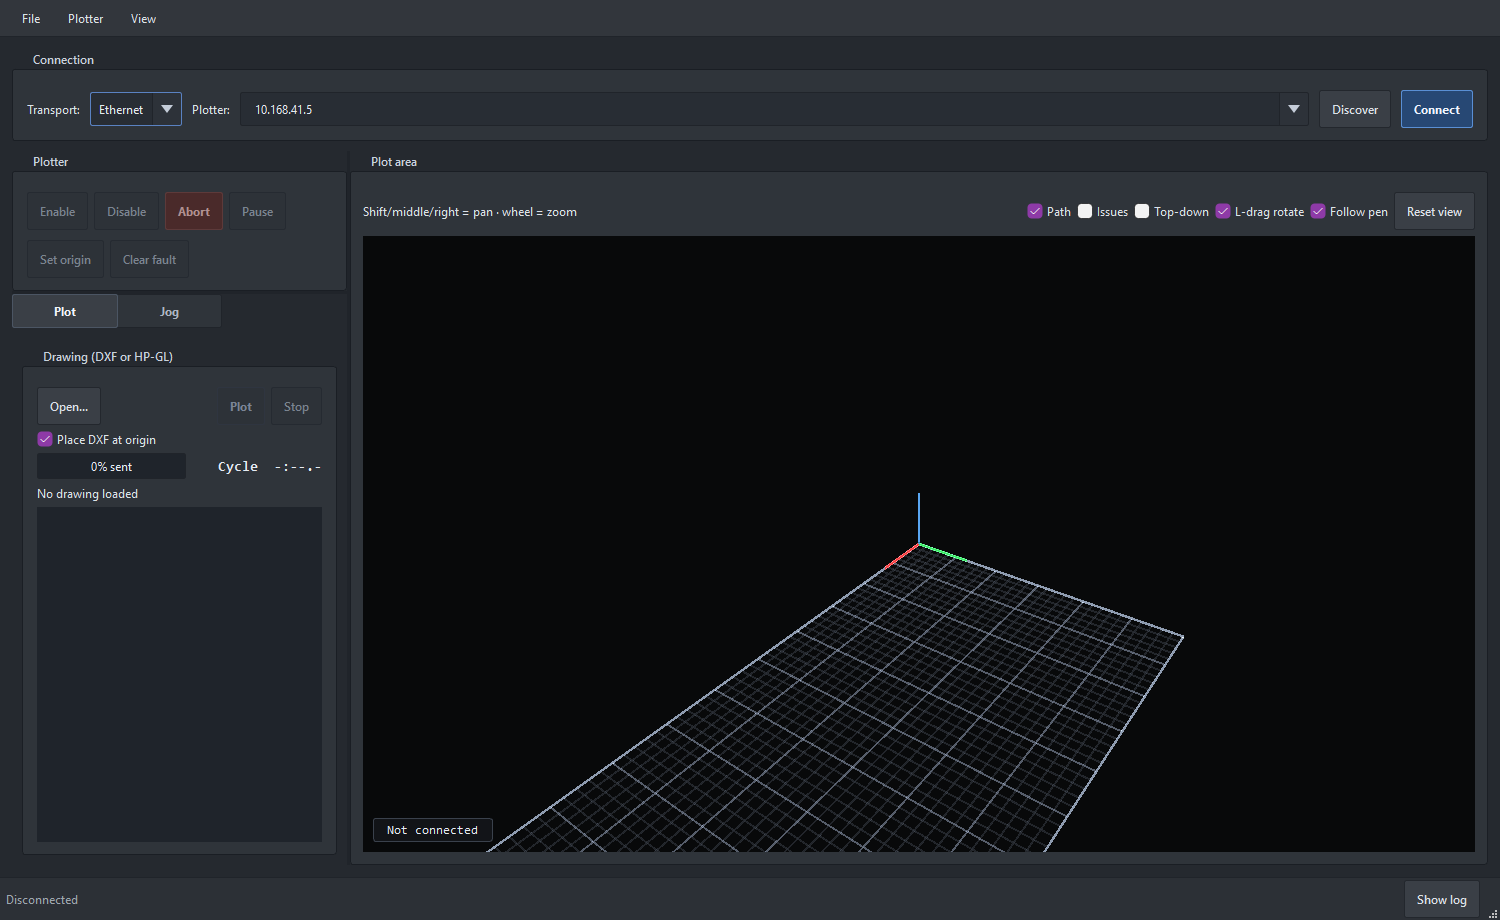
\includegraphics[width=\linewidth]{main-window.png}
\caption{The main window of the ClearHPGL app, before a connection}\label{fig:main}
\end{figure}

\section{Connect to the Plotter}

The app connects over Ethernet or over a serial port.

\begin{procedure}{Connect over Ethernet}
\begin{enumerate}
  \item Set \menu{Transport} to \menu{Ethernet}.
  \item Click \menu{Discover}. The app finds the boards on the local network
        and adds them to the \menu{Plotter} list.
  \item If the board is not found, type its IP address in \menu{Plotter}.
  \item Click \menu{Connect}.
\end{enumerate}
\end{procedure}

Over Ethernet, the app uses the console port (TCP 9300) for commands and
status, and the HP-GL port (TCP 9100) for jobs. The console port accepts one
client. While the app is connected, a terminal cannot use port 9300.

\begin{procedure}{Connect over a serial port}
\begin{enumerate}
  \item Set \menu{Transport} to \menu{Serial}.
  \item Click \menu{Refresh}, then select the COM port of the board.
  \item For the USB port, keep any baud rate and \menu{No flow control}.
  \item For \conn{COM-0} or \conn{COM-1}, set the baud rate to \key{com_baud}
        and the flow control to \key{com_handshake}.
  \item Click \menu{Connect}.
\end{enumerate}
\end{procedure}

When the app is connected, the status bar shows the state of the machine
(for example \code{idle}, \code{plotting}, or \code{fault}). The 3D view shows
the pen at its present position.

\section{Open a Drawing}

Click \menu{Open\ldots} on the \menu{Plot} tab, or use
\menu{File\,>\,Open drawing (DXF / HP-GL)\ldots}. The app opens two types of
file.

\subsection{HP-GL Files}

Files with the extension \file{.plt}, \file{.hpgl}, \file{.hgl}, \file{.hpg},
or \file{.prn}. The app sends the file to the board without changes. For the
preview, the app uses the HP-GL interpreter of the firmware. Thus the
position, the rotation, the scaling, and the clipping in the preview are the
same as on the machine.

\subsection{DXF Files}

The app reads ASCII DXF files. It reads these entities: \code{LINE},
\code{LWPOLYLINE}, \code{POLYLINE} (also with bulges), \code{ARC}, and
\code{CIRCLE}. It does not read binary DXF, text, splines, ellipses, or
blocks. In your CAD software, explode these objects into lines, arcs, and
polylines before you save the DXF.

\begin{caution}
The app uses the \code{\$INSUNITS} variable of the DXF to get the units. If
the DXF has no \code{\$INSUNITS}, or the value is 0 (unitless), the app uses
inches. Save the DXF with its units set, or the plot can be 25.4 times too
large or too small.
\end{caution}

The app prepares a DXF for plotting:

\begin{itemize}
  \item It joins lines whose ends touch into longer paths.
  \item It plots all shapes inside a closed contour before the contour.
        Thus holes are cut before the outline frees the part.
  \item It goes to the nearest shape next, to make the pen-up travel short.
  \item It sends arcs and circles as true arcs (HP-GL \cmd{AA}), not as
        short straight lines. The machine draws them as smooth curves.
\end{itemize}

When \menu{Place DXF at origin} is selected, the app moves the drawing so
that its lower-left corner is at plotter 0,0. Clear it to keep the
coordinates of the DXF.

\section{The 3D View}

The 3D view shows the bed as a grid with lines every \SI{10}{mm}. The drawing
is on the bed; pen-down lines and pen-up moves have different colors.

\begin{table}[htbp]
\centering
\caption{Controls of the 3D view}\label{tab:view}
\begin{tabularx}{\linewidth}{@{}P{0.3\linewidth}L@{}}
\toprule
\textbf{Control} & \textbf{Function} \\
\midrule
Mouse wheel & Zoom in and out. \\
Shift + drag, middle drag, or right drag & Move the view. \\
Left drag & Turn the view, when \menu{L-drag rotate} is selected. \\
\menu{Path} & Show or hide the drawing. \\
\menu{Issues} & Show or hide the markers for problems in the drawing. \\
\menu{Top-down} & Look straight down on the bed. \\
\menu{Follow pen} & Keep the pen in the center of the view while it plots. \\
\menu{Reset view} & Show the full drawing again. \\
\bottomrule
\end{tabularx}
\end{table}

\subsection{Problems in a Drawing}

When \menu{Issues} is selected, the view shows markers where the drawing can
give a bad result. Put the mouse on a marker to read the explanation. The app
finds these problems:

\begin{itemize}
  \item Contours that do not close (open profiles).
  \item Contours that almost touch across a pen-up move.
  \item Long pen-down jumps inside a path, and short gaps between long cuts.
  \item Corners so tight that the machine must slow down a lot.
  \item Lines that overlap or cross.
\end{itemize}

Right-click a marker for its menu. \menu{Copy explanation} and
\menu{Copy X, Y} copy the information. For a DXF, two quick fixes are
available:

\begin{description}[style=nextline,leftmargin=1.2em,font=\sffamily\bfseries\color{navy}]
  \item[Quick fix: close contour] Closes an open contour with a smooth bridge
        across the gap.
  \item[Quick fix: connect across pen-up] Joins two contours that almost touch
        into one path.
\end{description}

After a quick fix, the app orders the drawing again. Use
\menu{File\,>\,Save DXF geometry\ldots} to keep the repaired geometry in a
new DXF.

\section{Plot}

\begin{warning}
The machine moves when you click \menu{Plot}. Keep your hands out of the work
area.
\end{warning}

\begin{procedure}{Plot a drawing from the app}
\begin{enumerate}
  \item Connect to the plotter.
  \item Open the drawing.
  \item Look at the preview. Make sure that the drawing is in the plot area.
  \item Put the material and the pen on the machine.
  \item Click \menu{Plot}.
\end{enumerate}
\end{procedure}

Before the app sends a DXF job, it compares the drawing with the plot area of
the board. If shapes are outside the area, the app shows how many, and asks
you to continue or to stop. If the emergency stop input is open, the app does
not send the job.

During the plot:

\begin{itemize}
  \item The progress bar shows how much of the job the app has sent.
  \item The 3D view shows the pen, and paints the lines that are drawn in green.
  \item The HP-GL text below the progress bar highlights the instruction that
        the machine draws now.
  \item \menu{Cycle} shows the time from \menu{Plot} to the end of the plot.
\end{itemize}

The app also follows jobs from other programs. For example, when AutoCAD
plots on the USB port, the 3D view shows the pen and the lines that it draws.

\subsection{Pause and Stop}

\begin{description}[style=nextline,leftmargin=1.2em,font=\sffamily\bfseries\color{navy}]
  \item[Pause] The machine stops at the end of the segments in its queue and
        raises the pen. The button changes to \menu{Resume}. Click
        \menu{Resume} to lower the pen and continue.
  \item[Stop] The app stops sending and stops the plot on the board.
  \item[Abort] The board stops now, drops the job, and raises the pen. Use
        it for a job from any source.
\end{description}

\begin{warning}
\menu{Abort}, \menu{Stop}, and \menu{Pause} are not emergency stops. They
operate through the firmware and the link. Use the emergency stop if a person
or the machine is in danger.
\end{warning}

\section{Move the Pen}

The \menu{Jog} tab moves the pen with the pen up. The machine must not be
plotting.

\begin{itemize}
  \item \menu{Go to (pen up)}: type an X and a Y position in mm, then click
        \menu{Go}.
  \item \menu{Jog}: set \menu{Step (mm)}, then click \menu{X-}, \menu{X+},
        \menu{Y-}, or \menu{Y+}. The pen does not move out of the plot area.
  \item \menu{Pen up} and \menu{Pen down}: test the pen lift.
\end{itemize}

To make the present position the origin, click \menu{Set origin}.

\section{Plotter Settings}\label{sec:app-settings}

Use \menu{Plotter\,>\,Plotter settings\ldots} to change the settings of the
board. The app reads the settings from the board and shows them in groups
(figure~\ref{fig:settings}). Fixed choices are lists.

\begin{figure}[p]
\centering
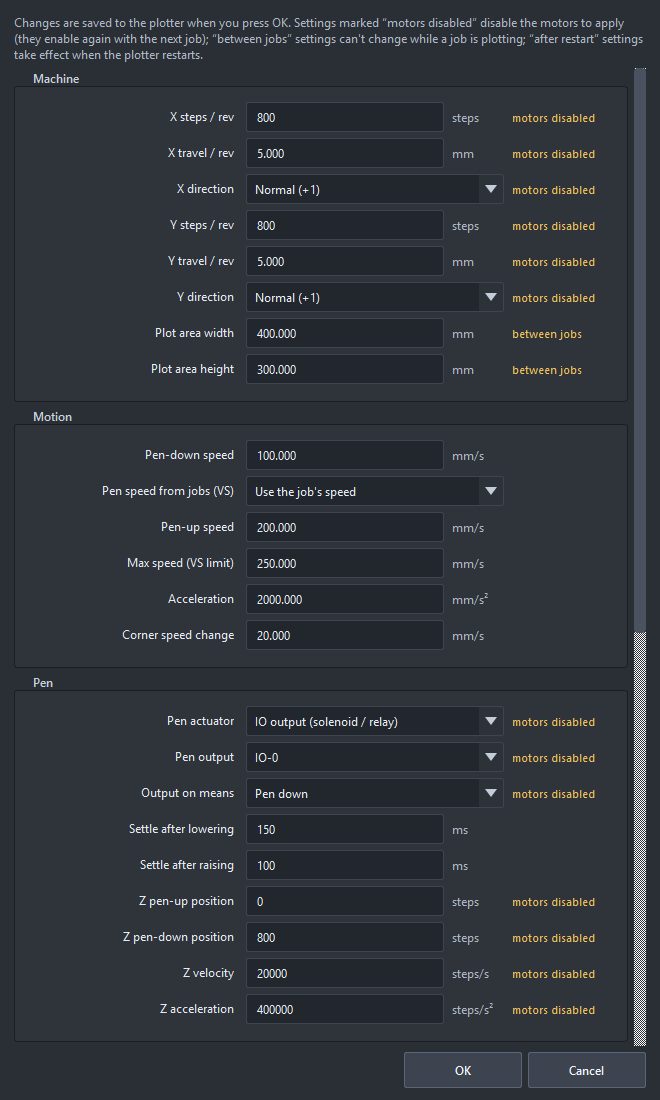
\includegraphics[width=0.78\linewidth]{settings-dialog.png}
\caption{The \menu{Plotter settings} dialog, with the factory settings}\label{fig:settings}
\end{figure}

A label next to a field tells you when the setting can change
(table~\ref{tab:when}):

\begin{description}[style=nextline,leftmargin=1.2em,font=\sffamily\bfseries\color{navy}]
  \item[motors disabled] The app disables the motors before it applies the
        change. The motors enable again with the next job.
  \item[between jobs] The change is not possible while a job plots, but the
        motors can stay enabled. The plot area has this label.
  \item[after restart] The board saves the change. It takes effect after the
        board restarts.
\end{description}

Click \menu{OK} to send the changes. The app does not send changes while a job
plots. If the board refuses a change, the app shows the settings that did not
change and the reason. The plot area of the app changes to the plot area of
the board.

\section{ClearPath Scope}\label{sec:scope}

\menu{Plotter\,>\,ClearPath scope\ldots} (Ctrl+Shift+O) records the signals
of the ClearPath servos through the USB port of each servo, the port that
ClearPath MSP uses. It shows them in lanes on one time axis
(figure~\ref{fig:scope}). Use it to see how the X and Y servos follow a plot:
the tracking error on each acceleration, the speed, the bus voltage, the
temperature, and the HLFB, enable, and alert signals.

The scope does not use the ClearCore. Thus it operates during a plot, and
over any link.

\begin{figure}[htbp]
\centering
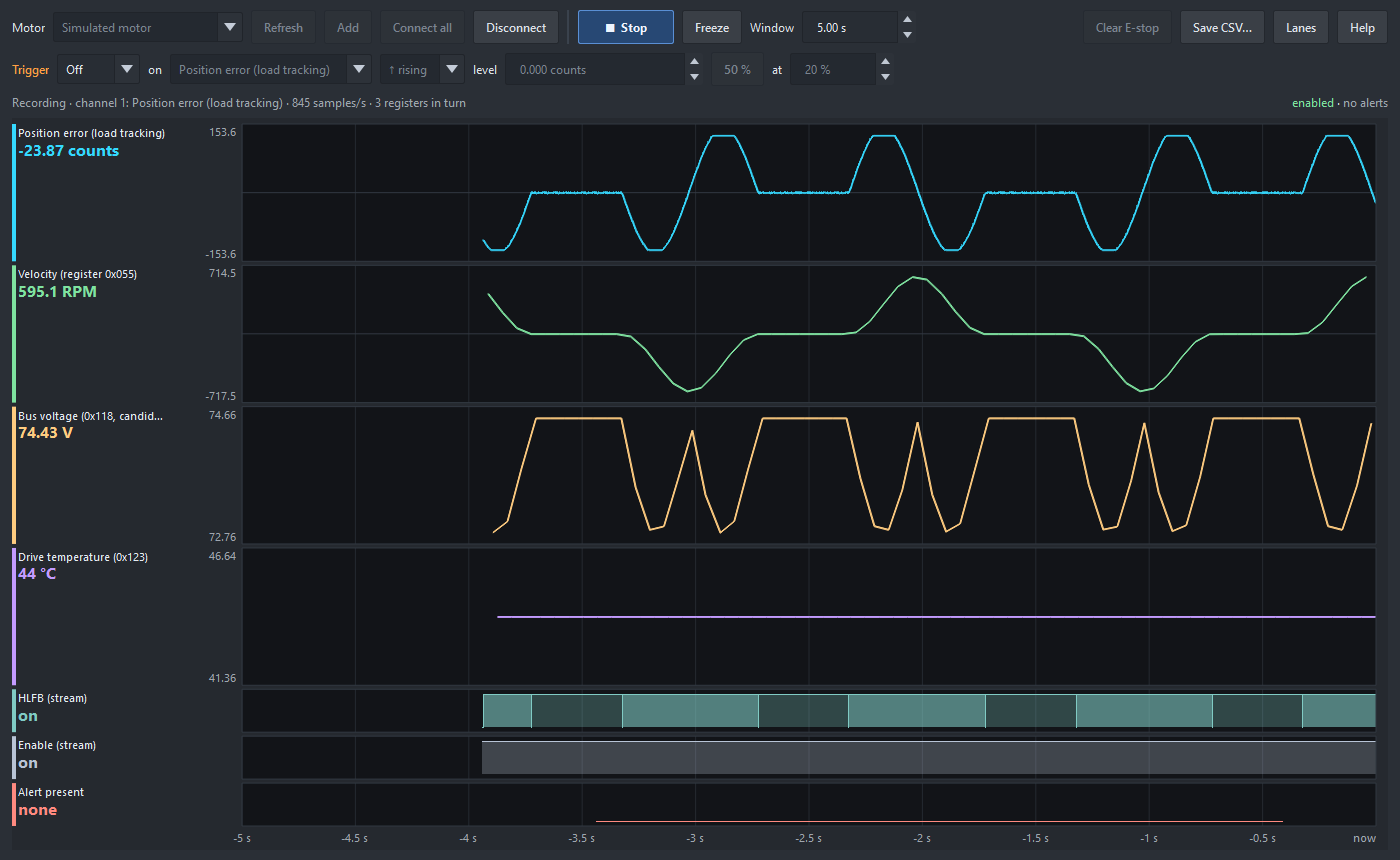
\includegraphics[width=\linewidth]{clearpath-scope.png}
\caption{The ClearPath scope, on its simulated motor}\label{fig:scope}
\end{figure}

\begin{procedure}{Record a ClearPath servo}
\begin{enumerate}
  \item Connect the USB port of the servo to the computer.
  \item Close ClearPath MSP. One program at a time can use the port.
  \item Select \menu{Plotter\,>\,ClearPath scope\ldots}.
  \item In \menu{Motor}, select the servo (\emph{ClearPath on COMn}). For more
        than one servo, click \menu{Connect all}.
  \item Click \menu{Connect}, then \menu{Start}.
  \item Click \menu{Stop} to stop the recording, then \menu{Disconnect}.
\end{enumerate}
\end{procedure}

\begin{itemize}
  \item \menu{Lanes} selects the signals, their sequence, color, and scale.
  \item \menu{Trigger} holds the screen on a repeated event, for example
        HLFB going low at the start of each move.
  \item \menu{Freeze} holds the view while the recording continues.
        \menu{Save CSV\ldots} saves the recording.
  \item \menu{Help} (F1) opens the full description of the scope.
  \item Without a servo, select \menu{Simulated motor} to try the scope.
\end{itemize}

\begin{note}
\notelabel The scope sets the working monitor channel of the servo while it
records, and sets it back when it stops. It saves nothing in the servo, and
it never enables or moves the motor.
\end{note}

\section{Other Functions}

\begin{itemize}
  \item \menu{File\,>\,Export HP-GL\ldots} saves the job as an HP-GL file. For a
        DXF, it is the HP-GL that the app sends.
  \item \menu{View\,>\,Command log} shows all commands and replies.
  \item \menu{View\,>\,Clear pen trace} removes the green trace of the last plot.
\end{itemize}

\chapter{Plot from CAD Software}\label{ch:cad}

The board operates like an HP plotter. Any program with an HP-GL or HP-GL/2
plotter driver can plot to it. You do not need the desktop app.

\section{AutoCAD}

AutoCAD has drivers for the HP DraftMaster plotters. Both of the drivers in
table~\ref{tab:acad} plot directly to the board.

\begin{table}[htbp]
\centering
\caption{AutoCAD drivers for ClearHPGL}\label{tab:acad}
\begin{tabularx}{\linewidth}{@{}P{0.3\linewidth}P{0.34\linewidth}L@{}}
\toprule
\textbf{Driver} & \textbf{Output} & \textbf{Setting on the board} \\
\midrule
DraftMaster RX 7596B (HP-GL/2), recommended & True arcs and compact encoded
polylines. The driver places the plot. & None. \\
Draftmaster 2 (7596A) (HP-GL) & Arcs as short lines. Plotter 0,0 is at the
center of the sheet. & \cmd{set ident 7596A} \\
\bottomrule
\end{tabularx}
\end{table}

\begin{procedure}{Set up an AutoCAD plotter for ClearHPGL}
\begin{enumerate}
  \item In AutoCAD, open the \menu{Add-a-Plotter} wizard.
  \item Select the manufacturer HP and the model \menu{DraftMaster RX 7596B}.
  \item Select the COM port of the board (the USB port or \conn{COM-0}/\conn{COM-1}).
  \item In \menu{Configure Port}, set the flow control to \menu{XON/XOFF}.
  \item Add a custom paper size that is the same as the plot area, with no
        margins.
  \item Plot a small drawing to test the setup.
\end{enumerate}
\end{procedure}

\begin{note}
\notelabel AutoCAD sends its own pen speed (\cmd{VS}) from its pen table.
To use the speed of the board, type \cmd{set job_speed 0}. Then the board
always uses \key{draw_mm_s} for the pen-down speed.
\end{note}

The path order of AutoCAD is not important. By default, the board keeps each
job from the USB port and the COM ports, and plots it in a better order
(section~\ref{sec:optimizer}).

\subsection{The Model Name}

The board replies to the HP-GL \cmd{OI} instruction with the model name in
\key{ident} (default \code{7475A}). Some drivers use this reply. The model
name also sets the position of plotter 0,0:

\begin{itemize}
  \item For \code{7475A}, \code{7550A}, and the other small models, plotter
        0,0 is the lower-left corner of the plot area.
  \item For the large DraftMaster models (\code{758x} and \code{759x}, for
        example \code{7596A}), plotter 0,0 is the center of the plot area.
        Their drivers send coordinates around the center.
\end{itemize}

Set \key{ident} to the model that your driver expects.

\section{Other Software}

Use a driver for an HP 7475A, an HP 7550A, or an HP DraftMaster. Most sign,
vinyl, and CAM programs have one of these drivers. Then:

\begin{itemize}
  \item Point the driver at the COM port of the board, or at TCP port 9100 of
        the board.
  \item On a COM port, use XON/XOFF flow control.
  \item Set the paper size to the plot area.
  \item Set the program to send text as lines. The board does not draw HP-GL
        text (\cmd{LB}).
\end{itemize}

Windows plotter drivers often put PCL or PJL commands around the HP-GL/2. The
board removes them.

\section{Send a File without a Driver}

You can send an HP-GL file directly to the board.

\begin{description}[style=nextline,leftmargin=1.2em,font=\sffamily\bfseries\color{navy}]
  \item[Windows, USB or COM port]
\begin{lstlisting}[language=console]
copy /b drawing.plt COM3
\end{lstlisting}
  \item[Linux or macOS, network]
\begin{lstlisting}[language=console]
nc 10.168.41.5 9100 < drawing.plt
\end{lstlisting}
  \item[Command-line client, any system with Python]
\begin{lstlisting}[language=console]
python Firmware/host/clearhpgl_cli.py discover
python Firmware/host/clearhpgl_cli.py --host 10.168.41.5 send drawing.plt
python Firmware/host/clearhpgl_cli.py --serial COM3 send drawing.plt
\end{lstlisting}
\end{description}

On the network, one connection to port 9100 is one job. The job ends when the
connection closes. Appendix~\ref{app:network} gives more information about
the command-line client.

\chapter{How the Board Processes a Job}\label{ch:jobs}

This chapter tells you what the board does with a job. Use it to understand
the result of a plot, and to set the board for your work.

\section{One Source at a Time}

The board receives HP-GL on three links: USB, COM, and TCP port 9100. One
source plots at a time. A source keeps the plotter until its buffer is empty
and the job has ended:

\begin{itemize}
  \item On TCP, the job ends when the connection closes.
  \item On USB and COM, the job ends when the source is quiet for 2~s.
\end{itemize}

Then the next source that has data starts. The other sources wait: TCP and
USB stop at the full buffer, and COM gets XOFF. The board sends the replies
to output instructions (for example \cmd{OI} or \cmd{OS}) to the source that
plots.

If the last instruction of a job has no \code{;}, the board ends it when the
job ends. For example, \code{PU0,0} at the end of a file operates.

\section{The Job Optimizer}\label{sec:optimizer}

CAD drivers often send a drawing in a bad order: an outline in many short
parts, or holes after the outline. The \term{job optimizer} of the board
keeps a full job and then plots it in a better order:

\begin{enumerate}
  \item It joins strokes whose ends touch into longer paths.
  \item It draws everything inside a closed contour before the contour. Thus
        outlines come last, and a cutter does not free a part before its
        holes are cut.
  \item From the shapes that are ready, it draws the nearest next. It starts
        a closed contour at its nearest vertex, and an open path at its
        nearer end.
\end{enumerate}

On the AutoCAD parts that were tested, the optimizer decreased the pen-up
travel by 45\%--65\%.

\subsection{Which Sources the Optimizer Changes}

The setting \key{optimize} selects the sources. Add the values of the
sources that you want:

\begin{table}[htbp]
\centering
\caption{Values of \key{optimize}}\label{tab:optimize}
\begin{tabularx}{\linewidth}{@{}P{0.12\linewidth}L@{}}
\toprule
\textbf{Value} & \textbf{Source} \\
\midrule
1 & USB \\
2 & COM-0 or COM-1 \\
4 & Network (TCP 9100) \\
\bottomrule
\end{tabularx}
\end{table}

The default is 3 (USB and COM), because CAD drivers use these links. The
desktop app orders its own jobs, so the board does not change network jobs.

\subsection{What the Optimizer Changes}

\begin{itemize}
  \item The plot starts only when the job ends. While the board keeps the
        job, \cmd{status} shows \code{state=buffering}.
  \item A pen change or a speed change divides a job into groups. The groups
        keep their sequence.
  \item A page break (\cmd{PG}) ends a page. The board plots each page when
        it ends.
  \item A page can have 8000 points and 500 strokes. A larger job plots in
        the sequence that it arrives, and the remainder streams through.
  \item Arcs in a job that the optimizer changes are drawn as short lines
        (chords).
\end{itemize}

The \cmd{diag} command shows the last job: the number of strokes and paths,
and the pen-up travel before and after the optimizer.

\section{Arcs and Circles}

The HP-GL instructions for arcs and circles are \cmd{AA}, \cmd{AR},
\cmd{CI}, \cmd{EW}, and \cmd{WG}. With the pen down, the board draws each one
as a \term{true arc}: one smooth movement on the circle. The speed on an arc
is limited, so that the acceleration toward the center stays in
\key{accel_mm_s2}. The \cmd{status} command counts the arcs (\code{arcs=}).

The board draws an arc as \term{chords} (short straight lines) when:

\begin{itemize}
  \item the optimizer changes the job (\key{optimize}),
  \item the job scales X and Y differently, so the circle is an ellipse,
  \item the arc goes out of the clip window or the plot area,
  \item X and Y have different steps per millimeter, or
  \item the radius is less than a few motor steps.
\end{itemize}

Chords are 5° by default. The job can set a different angle with the chord
parameter, or set a maximum deviation with \cmd{CT1}. The minimum is 0.5°.

\section{Speed}

\begin{itemize}
  \item With the pen up, the speed is \key{travel_mm_s}.
  \item With the pen down, the speed is \key{draw_mm_s}. With \key{job_speed}~1,
        the \cmd{VS} instruction of a job sets it (in cm/s), up to \key{max_mm_s}.
        \cmd{VS} without a value sets it back to \key{draw_mm_s}.
  \item On curves, the board decreases the speed. The acceleration toward the
        center of the curve stays in \key{accel_mm_s2}. This applies to true
        arcs and to curves made of short lines.
  \item At a corner, the speed of each axis changes by no more than
        \key{corner_mm_s}.
\end{itemize}

The planner looks ahead along the segments in its queue and always plans to
stop at the last one. If the computer sends data too slowly, the machine
slows down. It does not lose its position.

\section{Coordinates and Clipping}

\begin{itemize}
  \item One plotter unit is \SI{0.025}{mm} (40 units per mm).
  \item The plot area is \key{width_mm} by \key{height_mm}, from plotter 0,0.
  \item The board moves the pen up to the edge of the plot area, not past it.
  \item A pen-down line is clipped to the clip window (\cmd{IW}) and to the
        plot area. The pen goes up where a line leaves the window and down
        where it comes back.
  \item A point that is less than half a plotter unit (\SI{0.0125}{mm})
        outside the plot area is on the edge. A drawing that touches the edge
        of the plot area plots without a pen lift.
  \item \cmd{RO} rotates the coordinates by 90°, 180°, or 270°.
\end{itemize}

\section{Pen Changes}

The board raises and lowers the pen only when the axes are stopped. After a
pen change, it waits for the settle time (\key{pen_down_ms} or
\key{pen_up_ms}). Between two pen changes, the segments flow through the
planner without a stop.

\section{Abort a Job}

These actions stop a job, drop the data that the board has kept, and raise
the pen:

\begin{itemize}
  \item The console command \cmd{abort}, or \menu{Abort} in the app.
  \item The device-control sequence \code{ESC.K} from the source that plots.
\end{itemize}

After a fault, the board also drops the job. A TCP job is closed. A serial
job is discarded until its source is quiet for 2~s, so the remainder of the
job does not plot.

\chapter{Troubleshooting}\label{ch:trouble}

\section{Read the State of the Board}

The \cmd{status} command shows the state of the machine. The desktop app
shows the same data in its status bar and its log. This is an example:

\begin{lstlisting}[language=console]
state=idle enabled=1 x_mm=0.000 y_mm=0.000 pen=up sel_pen=1 queue=0
planner=0 segments=1767 arcs=550 arc_fallbacks=0 curve_capped=1298
dropped=0 pages=0 estop=ok fault=none
\end{lstlisting}

\begin{table}[htbp]
\centering
\caption{Fields of \cmd{status}}\label{tab:status}
\begin{tabularx}{\linewidth}{@{}P{0.24\linewidth}L@{}}
\toprule
\textbf{Field} & \textbf{Meaning} \\
\midrule
\code{state} & \code{idle}, \code{buffering} (the optimizer keeps a job),
\code{plotting}, \code{paused}, \code{disabled}, \code{waiting_enable}, or
\code{fault}. \\
\code{enabled} & 1 if the motors are enabled. \\
\code{x_mm}, \code{y_mm}, \code{pen} & The position of the pen and its state. \\
\code{queue}, \code{planner} & Actions that wait in the board, and segments in the planner. \\
\code{segments}, \code{arcs} & Lines and true arcs sent to the planner since power-up. \\
\code{arc_fallbacks} & Arcs that the planner refused and that the board drew as a line. \\
\code{curve_capped} & Segments that were slower because of a curve. \\
\code{dropped} & Segments that the board could not plot (for example, zero length). \\
\code{estop}, \code{fault} & The emergency stop input, and the latched fault. \\
\bottomrule
\end{tabularx}
\end{table}

The second line of \cmd{status} shows the links: the bytes received on each
link, the source that plots, the IP address, and the counters of HP-GL
instructions, unknown instructions, and skipped labels.

\section{Faults}

A fault stops the machine (section~\ref{sec:fault-behavior}). The
\code{fault} field tells you the cause.

\begin{table}[htbp]
\centering
\caption{Faults}\label{tab:faults}
\begin{tabularx}{\linewidth}{@{}P{0.32\linewidth}L@{}}
\toprule
\textbf{Fault} & \textbf{Action} \\
\midrule
\code{estop (DI-6)} & Close the emergency stop. Examine the wiring of
\conn{DI-6}. If no emergency stop is connected, set \key{estop_di6}~0. \\
\code{motor fault on M0 (X)}, \code{motor fault on M1 (Y)} & Examine the
servo with ClearPath MSP: tracking error, overload, or power. Then type
\cmd{clear}. \\
\code{HLFB not asserted} & A servo does not supply its ready signal. Examine
its power, its cable, and its HLFB setting in MSP. Set \key{hlfb_check}~0 only
if your servos have no HLFB. \\
\code{pen Z move timed out} & The pen servo on \conn{M2} did not finish its
move in 5~s. Examine the servo and \key{z_vel_steps}. \\
\bottomrule
\end{tabularx}
\end{table}

To clear a fault, remove the cause, then type \cmd{clear} or click
\menu{Clear fault}. The \cmd{enable} command also clears it.

\section{Diagnostics}

The \cmd{diag} command shows information about the motion. The command
\cmd{diag reset} sets the timing counters to zero first.

\begin{lstlisting}[language=console]
bursts=0 (samples asking > 16 steps) excess_carried M0=0 M1=0
timing: max_irq_off=0 us (QueueLinear/QueueArc) max_update_gap=212 us ...
step interrupt: max=93 us (arc start)  slow(>150us of 200)=0
controller x=68900 y=15239  pulses_sent M0=68900 M1=15239
optimizer: idle  last job: 3 strokes -> 3 paths, pen-up travel 136 -> 127 mm
\end{lstlisting}

\begin{description}[style=nextline,leftmargin=1.2em,font=\sffamily\bfseries\color{navy}]
  \item[bursts] Samples that asked for more than 16 steps. It must be 0.
  \item[step interrupt] The longest time of the step interrupt, and how many
        times it used more than \SI{150}{\micro s} of its \SI{200}{\micro s}
        period. If the interrupt is too long, a motor can jump. A value near
        \SI{200}{\micro s} is a problem.
  \item[controller, pulses\_sent] The position of the planner and the pulses
        sent to each motor. They must be the same.
  \item[optimizer] The last job: strokes, paths, and the pen-up travel before
        and after the optimizer.
\end{description}

\section{Problems and Remedies}

\begin{longtable}{@{}P{0.33\linewidth}P{0.62\linewidth}@{}}
\caption{Problems and remedies}\label{tab:problems}\\
\toprule
\textbf{Problem} & \textbf{Possible cause and remedy} \\
\midrule
\endfirsthead
\toprule
\textbf{Problem} & \textbf{Possible cause and remedy} \\
\midrule
\endhead
\bottomrule
\endfoot
Nothing plots from the USB port & The console is open: type \cmd{exit}.
The optimizer keeps the job until the port is quiet for 2~s: wait. A fault
is latched: read \cmd{status}. \\
The state stays \code{waiting_enable} & \key{auto_enable} is 0. Type
\cmd{enable}, or set \key{auto_enable}~1. \\
The motors do not enable & The emergency stop is open, or HLFB is missing.
Read the fault. \\
The board is not found on the network & The board uses 192.168.0.110 if DHCP
fails. Make sure that the computer is on the same subnet. Type \cmd{status}
on the USB console to read the \code{ip} field. \\
A terminal cannot connect to port 9300 & The console accepts one client. Close
the desktop app or the other terminal. \\
The plot has the wrong size & Examine \key{steps_rev_x}, \key{mm_rev_x},
\key{steps_rev_y}, and \key{mm_rev_y}. For a DXF, examine its units
(\code{\$INSUNITS}). \\
The plot is mirrored & Set \key{dir_x} or \key{dir_y} to -1. \\
The plot is at the wrong position & Set the origin again. For an AutoCAD
DraftMaster driver, examine \key{ident} and the paper size. \\
Parts of the drawing are missing & The drawing is outside the plot area.
Text (\cmd{LB}) is not drawn: send text as lines. \\
The pen moves before it is down & Increase \key{pen_down_ms}. \\
Corners are rough, or the machine shakes & Decrease \key{accel_mm_s2} or
\key{corner_mm_s}. \\
The machine is slow on small curves & This is correct: the speed on a curve is
limited by \key{accel_mm_s2}. Increase it if the machine can accelerate more. \\
Arcs look like polygons & The job came through the optimizer, or the axes
have different scales. Read the causes in chapter~\ref{ch:jobs}. \\
A motor jumps & Type \cmd{diag}. Examine \code{step interrupt} and
\code{pulses_sent}. Report the values with the job that caused the jump. \\
\code{error: disable motors first} & The setting needs the motors disabled.
Type \cmd{disable}. \\
\code{error: a job is running} & The setting can change only between jobs.
Wait until the job ends. \\
\code{applied but NVM write failed} & The supply voltage is too low to write
the memory. Connect the 24~V supply and set the value again. \\
\end{longtable}


\appendix
\chapter{Console Commands}\label{app:console}

The console is on the USB port (type \cmd{menu} on a line by itself) and on
TCP port 9300. Each command ends with a line that starts with \code{ok} or
\code{error:}. When the console opens, it shows the firmware version, the
model name, the IP address, the active links, and the source of the
settings.

\begin{longtable}{@{}P{0.27\linewidth}P{0.68\linewidth}@{}}
\caption{Console commands}\label{tab:console}\\
\toprule
\textbf{Command} & \textbf{Function} \\
\midrule
\endfirsthead
\toprule
\textbf{Command} & \textbf{Function} \\
\midrule
\endhead
\bottomrule
\endfoot
\cmd{help}, \cmd{menu} & Show the list of commands. \\
\cmd{status} & Show the state, the position in mm, the pen, the queue depth,
the counters, and the data of the links (table~\ref{tab:status}). \\
\cmd{config} & Show all settings with their values, their descriptions, and
when they take effect. \\
\cmd{set} \textit{key value} & Make sure that the value is correct, apply it,
and save it in the nonvolatile memory. Appendix~\ref{app:settings} lists the
keys. \\
\cmd{defaults} & Set all settings to the factory values. The motors must be
disabled. \\
\cmd{enable} & Enable the motors. This also clears a latched fault. With
\key{hlfb_check}~1, the board waits for HLFB from all servos. \\
\cmd{disable} & Disable the motors. A job that is in the queue is dropped. \\
\cmd{abort} & Stop now, drop the job, and raise the pen. \\
\cmd{pause} & Stop at the end of the segments in the queue, and raise the pen. \\
\cmd{resume} & Lower the pen and continue after \cmd{pause}. \\
\cmd{origin} & The present position becomes plotter 0,0. No job can be
plotting. \\
\cmd{goto} \textit{x\_mm y\_mm} & Move to the position with the pen up. No job
can be plotting. The position stays in the plot area. \\
\cmd{pen up}, \cmd{pen down} & Raise or lower the pen to test it. No job can
be plotting. \\
\cmd{clear} & Clear a latched fault. Remove the cause first. \\
\cmd{diag} & Show the motion diagnostics, the last job of the optimizer, and
the data of the USB link. \\
\cmd{diag reset} & Set the timing counters to zero, then show the diagnostics. \\
\cmd{tel} \textit{ms} & TCP console only. Send a line \code{TEL ms= x= y= pen=
state= queue=} every \textit{ms} milliseconds (10 or more; 0 stops it). A line
is sent only when the TCP buffer has space, so a slow client cannot stop the
motion. The desktop app uses 25~ms. \\
\cmd{restart} & Restart the board. \\
\cmd{version} & Show the name and the version of the firmware. \\
\cmd{exit}, \cmd{quit}, \cmd{q} & Close the console. On USB, the port goes back
to HP-GL. \\
\end{longtable}

\section*{Error Messages}

\begin{table}[htbp]
\centering
\caption{Common console errors}\label{tab:console-errors}
\begin{tabularx}{\linewidth}{@{}P{0.45\linewidth}L@{}}
\toprule
\textbf{Message} & \textbf{Meaning} \\
\midrule
\code{unknown key (try: config)} & The setting name is not correct. \\
\code{disable motors first} & The setting needs the motors disabled. \\
\code{a job is running; change it when the plotter is idle} & The setting can change only between jobs. \\
\code{applied but NVM write failed} & The board uses the value but could not save it. The supply voltage is too low. \\
\code{plotter busy} & The command needs the machine to be idle. \\
\code{unknown command (try: help)} & The command name is not correct. \\
\bottomrule
\end{tabularx}
\end{table}

\chapter{Settings}\label{app:settings}

The board keeps its settings in nonvolatile memory. Change a setting with
\cmd{set} \textit{key value} in the console, or in \menu{Plotter settings} in
the desktop app. \cmd{config} shows all values. \cmd{defaults} sets the
factory values.

The column ``When'' tells you when a change is possible
(table~\ref{tab:when}): \textbf{live} (at any time), \textbf{idle} (between
jobs), \textbf{disabled} (with the motors disabled), or \textbf{restart}
(after \cmd{restart}).

\section{Machine}

\begin{longtable}{@{}P{0.2\linewidth}P{0.11\linewidth}P{0.16\linewidth}P{0.1\linewidth}P{0.33\linewidth}@{}}
\caption{Machine settings}\label{tab:set-machine}\\
\toprule
\textbf{Key} & \textbf{Default} & \textbf{Range} & \textbf{When} & \textbf{Function} \\
\midrule
\endfirsthead
\toprule
\textbf{Key} & \textbf{Default} & \textbf{Range} & \textbf{When} & \textbf{Function} \\
\midrule
\endhead
\bottomrule
\endfoot
\key{kinematics} & 0 & 0 or 1 & disabled & 0: Cartesian (\conn{M0} = X, \conn{M1} = Y). 1: CoreXY or H-bot (\conn{M0} = A, \conn{M1} = B). Section~\ref{sec:corexy}. A change sets the origin. \\
\key{steps_rev_x} & 800 & 1--1,000,000 & disabled & \conn{M0} steps per revolution. \\
\key{steps_rev_y} & 800 & 1--1,000,000 & disabled & \conn{M1} steps per revolution. CoreXY: the same as \conn{M0}. \\
\key{mm_rev_x} & 5.0 & 0.001--10,000 & disabled & Cartesian: X travel per motor revolution, mm. \\
\key{mm_rev_y} & 5.0 & 0.001--10,000 & disabled & Cartesian: Y travel per motor revolution, mm. \\
\key{pulley_dia_mm} & 12.7324 & 0.1--1000 & disabled & CoreXY: pulley pitch diameter, mm, both motors. Travel per revolution is $\pi$ $\times$ this value. \\
\key{dir_x} & 1 & 1 or -1 & disabled & Direction of X. -1 reverses it. \\
\key{dir_y} & 1 & 1 or -1 & disabled & Direction of Y. -1 reverses it. \\
\key{swap_xy} & 0 & 0 or 1 & disabled & 1: exchange the X and Y axes. A change sets the origin. \\
\key{width_mm} & 400 & 1--100,000 & idle & Plot area in X (the hard clip), mm. \\
\key{height_mm} & 300 & 1--100,000 & idle & Plot area in Y (the hard clip), mm. \\
\end{longtable}

\section{Motion}

\begin{longtable}{@{}P{0.2\linewidth}P{0.11\linewidth}P{0.16\linewidth}P{0.1\linewidth}P{0.33\linewidth}@{}}
\caption{Motion settings}\label{tab:set-motion}\\
\toprule
\textbf{Key} & \textbf{Default} & \textbf{Range} & \textbf{When} & \textbf{Function} \\
\midrule
\endfirsthead
\toprule
\textbf{Key} & \textbf{Default} & \textbf{Range} & \textbf{When} & \textbf{Function} \\
\midrule
\endhead
\bottomrule
\endfoot
\key{draw_mm_s} & 100 & 0.1--10,000 & live & Pen-down speed, mm/s. \cmd{VS} without a value sets it back to this value. \\
\key{travel_mm_s} & 200 & 0.1--10,000 & live & Pen-up speed, mm/s. \\
\key{max_mm_s} & 250 & 0.1--10,000 & live & Highest speed that \cmd{VS} can set, mm/s. \\
\key{job_speed} & 1 & 0 or 1 & live & 1: \cmd{VS} in a job sets the pen-down speed. 0: always \key{draw_mm_s}. \\
\key{accel_mm_s2} & 2000 & 1--1,000,000 & live & Acceleration along the path, mm/s\textsuperscript{2}. Also limits the speed on curves. \\
\key{corner_mm_s} & 20 & 0--10,000 & live & Largest change of speed of one motor at a corner, mm/s. \\
\key{motor_max_mm_s} & 0 & 0--10,000 & live & Highest speed of a motor, as belt travel in mm/s. 0: no limit. Use it for CoreXY. \\
\end{longtable}

\section{Pen}

\begin{longtable}{@{}P{0.2\linewidth}P{0.11\linewidth}P{0.16\linewidth}P{0.1\linewidth}P{0.33\linewidth}@{}}
\caption{Pen settings}\label{tab:set-pen}\\
\toprule
\textbf{Key} & \textbf{Default} & \textbf{Range} & \textbf{When} & \textbf{Function} \\
\midrule
\endfirsthead
\toprule
\textbf{Key} & \textbf{Default} & \textbf{Range} & \textbf{When} & \textbf{Function} \\
\midrule
\endhead
\bottomrule
\endfoot
\key{pen_mode} & 0 & 0 or 1 & disabled & 0: digital output. 1: servo on \conn{M2}. \\
\key{pen_io} & 0 & 0--5 & disabled & Output for the pen, \conn{IO-0}--\conn{IO-5} (\key{pen_mode}~0). \\
\key{pen_active_high} & 1 & 0 or 1 & disabled & 1: the output is on when the pen is down. \\
\key{pen_down_ms} & 150 & 0--10,000 & live & Settle time after the pen goes down, ms. \\
\key{pen_up_ms} & 100 & 0--10,000 & live & Settle time after the pen goes up, ms. \\
\key{z_up_steps} & 0 & $\pm$100,000,000 & disabled & \conn{M2} pen-up position, steps. \\
\key{z_down_steps} & 800 & $\pm$100,000,000 & disabled & \conn{M2} pen-down position, steps. \\
\key{z_vel_steps} & 20,000 & 1--10,000,000 & disabled & \conn{M2} speed, steps/s. \\
\key{z_accel_steps} & 400,000 & 1--100,000,000 & disabled & \conn{M2} acceleration, steps/s\textsuperscript{2}. \\
\end{longtable}

\section{Safety and Jobs}

\begin{longtable}{@{}P{0.2\linewidth}P{0.11\linewidth}P{0.16\linewidth}P{0.1\linewidth}P{0.33\linewidth}@{}}
\caption{Safety and job settings}\label{tab:set-safety}\\
\toprule
\textbf{Key} & \textbf{Default} & \textbf{Range} & \textbf{When} & \textbf{Function} \\
\midrule
\endfirsthead
\toprule
\textbf{Key} & \textbf{Default} & \textbf{Range} & \textbf{When} & \textbf{Function} \\
\midrule
\endhead
\bottomrule
\endfoot
\key{estop_di6} & 1 & 0--2 & live & 0: off. 1: fault when \conn{DI-6} is low. 2: fault when it is high. \\
\key{auto_enable} & 1 & 0 or 1 & live & 1: enable the motors when a job arrives. \\
\key{hlfb_check} & 1 & 0 or 1 & live & 1: the servos must supply HLFB when the motors enable. \\
\key{optimize} & 3 & 0--7 & live & Sources that the optimizer orders: 1 USB, 2 COM, 4 network. Add the values. \\
\key{ident} & \code{7475A} & text & live & Reply to \cmd{OI}. \code{758x} and \code{759x} (DraftMaster) put plotter 0,0 at the center of the bed. \\
\end{longtable}

\section{Serial Port and Network}

\begin{longtable}{@{}P{0.2\linewidth}P{0.11\linewidth}P{0.16\linewidth}P{0.1\linewidth}P{0.33\linewidth}@{}}
\caption{Serial port and network settings}\label{tab:set-links}\\
\toprule
\textbf{Key} & \textbf{Default} & \textbf{Range} & \textbf{When} & \textbf{Function} \\
\midrule
\endfirsthead
\toprule
\textbf{Key} & \textbf{Default} & \textbf{Range} & \textbf{When} & \textbf{Function} \\
\midrule
\endhead
\bottomrule
\endfoot
\key{com_port} & 0 & 0--2 & restart & HP-GL serial port. 0: off. 1: \conn{COM-0}. 2: \conn{COM-1}. \\
\key{com_baud} & 9600 & 300--1,000,000 & restart & Baud rate of the serial port. \\
\key{com_handshake} & 1 & 0--2 & restart & 0: none. 1: XON/XOFF. 2: RTS/CTS. \\
\key{com_rs232} & 1 & 0 or 1 & restart & 1: RS-232 levels. 0: TTL levels. \\
\key{net_mode} & 0 & 0 or 1 & restart & 0: DHCP. 1: static address. \\
\key{ip} & -- & address & restart & Static IP address. \\
\key{netmask} & -- & address & restart & Static netmask. \\
\key{gateway} & -- & address & restart & Static gateway. \\
\end{longtable}

\begin{note}
\notelabel With DHCP, if the board gets no address, it uses 192.168.0.110.
\end{note}

\chapter{HP-GL Support}\label{app:hpgl}

The board operates as an HP-GL pen plotter of the HP 7475A class. It also
reads the HP-GL/2 instructions that drivers usually send. The HP-GL/2
reference guide gives the full definition of each
instruction.\footnote{Hewlett-Packard Company, \textit{The HP-GL/2 and HP RTL
Reference Guide: A Handbook for Program Developers}, 3rd ed. (Reading, MA:
Addison-Wesley, 1997).}

\section{Syntax}

\begin{itemize}
  \item Mnemonics are not case sensitive.
  \item Commas or spaces separate parameters.
  \item An instruction ends with \code{;} or with the next mnemonic, for
        example \code{PA10,10PD20,20}.
  \item Decimal values and signs are correct in all parameters.
\end{itemize}

\section{Instructions}

\begin{longtable}{@{}P{0.16\linewidth}P{0.34\linewidth}P{0.45\linewidth}@{}}
\caption{HP-GL instructions}\label{tab:hpgl}\\
\toprule
\textbf{Group} & \textbf{Instructions} & \textbf{Notes} \\
\midrule
\endfirsthead
\toprule
\textbf{Group} & \textbf{Instructions} & \textbf{Notes} \\
\midrule
\endhead
\bottomrule
\endfoot
Setup & \cmd{IN} \cmd{DF} \cmd{IP} \cmd{IR} \cmd{SC} (types 0, 1, and 2) \cmd{IW} \cmd{RO} &
\cmd{IN} raises the pen, sets P1 and P2 to the plot area, and clears errors. \\
Pen and motion & \cmd{PU} \cmd{PD} \cmd{PA} \cmd{PR} \cmd{PE} &
\cmd{PE} is the HP-GL/2 encoded polyline, with all its flags (base 64, 7-bit,
fractional bits, absolute, pen up, and pen select). \\
Pen and speed & \cmd{SP} \cmd{VS} &
One pen. \cmd{SP0} raises the pen. \cmd{VS} is in cm/s, up to \key{max_mm_s}. \\
Arcs and shapes & \cmd{AA} \cmd{AR} \cmd{CI} \cmd{CT} \cmd{EA} \cmd{ER}
\cmd{EW} \cmd{RA} \cmd{RR} \cmd{WG} \cmd{XT} \cmd{YT} \cmd{TL} &
Pen-down arcs are true arcs. \cmd{CI} and \cmd{EW} go back to the center.
\cmd{RA}, \cmd{RR}, and \cmd{WG} draw only the outline. \\
Page & \cmd{PG} \cmd{NR} \cmd{AF} \cmd{AH} \cmd{FR} & Raise the pen and count a page. \\
Output & \cmd{OI} \cmd{OS} \cmd{OE} \cmd{OA} \cmd{OC} \cmd{OP} \cmd{OH}
\cmd{OW} \cmd{OF} \cmd{OO} \cmd{OT} \cmd{OD} \cmd{OG} \cmd{OL} &
\cmd{OI} replies with \key{ident}. \cmd{OS} clears bits 8 and 2 after it is
read. \cmd{OE} clears the error. \\
Text & \cmd{LB} \cmd{DT} & Not drawn. The board reads the text up to the
terminator and counts it. \\
No effect & \cmd{LT} \cmd{PT} \cmd{FT} \cmd{LA} \cmd{PW} \cmd{WU} \cmd{NP}
\cmd{PC} \cmd{BP} \cmd{PS} \cmd{QL} \cmd{RP} \cmd{MC} \cmd{CO} \cmd{MG}
\cmd{SI} \cmd{SR} \cmd{DI} \cmd{DR} \cmd{CS} \cmd{CA} \cmd{SS} \cmd{SA}
\cmd{ES} \cmd{LO} \cmd{CP} \cmd{SM}, and others &
Accepted and ignored. All lines are solid. Strings in quotes are skipped. \\
\end{longtable}

An instruction that is not in table~\ref{tab:hpgl} sets error 1 and is
skipped. The board removes \code{@PJL} lines and the PCL and PJL escape
sequences that Windows drivers send.

\section{Errors and Status}

\begin{table}[htbp]
\centering
\caption{Error codes (\cmd{OE})}\label{tab:oe}
\begin{tabularx}{\linewidth}{@{}P{0.12\linewidth}L@{}}
\toprule
\textbf{Code} & \textbf{Meaning} \\
\midrule
0 & No error. \\
1 & Instruction not known. \\
2 & Wrong number of parameters. \\
3 & Parameter not correct (for example \code{RO45}, or \cmd{SC} with a range of zero). \\
6 & Position overflow. \\
\bottomrule
\end{tabularx}
\end{table}

\begin{table}[htbp]
\centering
\caption{Status bits (\cmd{OS})}\label{tab:os}
\begin{tabularx}{\linewidth}{@{}P{0.1\linewidth}P{0.1\linewidth}L@{}}
\toprule
\textbf{Bit} & \textbf{Value} & \textbf{Meaning} \\
\midrule
0 & 1 & Pen down. \\
1 & 2 & P1 or P2 changed (cleared by \cmd{OS} or \cmd{OP}). \\
3 & 8 & Initialized (set by \cmd{IN}, cleared by \cmd{OS}). \\
4 & 16 & Ready. \\
5 & 32 & Error (cleared by \cmd{OE}). \\
\bottomrule
\end{tabularx}
\end{table}

At power-up, \cmd{OS} replies 24.

\section{Device Control (ESC~.)}

The board answers these sequences immediately, before the data in its
buffer, as an HP 7475A does. They operate on all links. The reply ends with a
carriage return; \code{ESC.M} can change this.

\begin{longtable}{@{}P{0.3\linewidth}P{0.65\linewidth}@{}}
\caption{Device-control sequences}\label{tab:esc}\\
\toprule
\textbf{Sequence} & \textbf{Function or reply} \\
\midrule
\endfirsthead
\toprule
\textbf{Sequence} & \textbf{Function or reply} \\
\midrule
\endhead
\bottomrule
\endfoot
\code{ESC.(} \code{ESC.Y} & Plotter on. \\
\code{ESC.)} \code{ESC.Z} & Plotter off. The board discards data until the plotter is on. \\
\code{ESC.B} & Free bytes in the buffer. \\
\code{ESC.L} & Size of the buffer. \\
\code{ESC.O} & 8 if the buffer is empty, or 0. \\
\code{ESC.E} & Extended error, then clear it: 11 bad byte after \code{ESC.}, 12 bad
parameter, 14 too many parameters, 16 buffer overflow. \\
\code{ESC.K} & Stop the graphics: drop the buffered data, stop the motion, and raise the pen. \\
\code{ESC.J} & Stop device control (cancel an ACK that waits). \\
\code{ESC.R} & Reset the handshake and the output settings. \\
\code{ESC.H}, \code{ESC.I} & ENQ/ACK handshake. \\
\code{ESC.N} & Enable XON/XOFF with the given XOFF character. \\
\code{ESC.M} & Set the output terminator. \\
\code{ESC.@} \code{ESC.S} \code{ESC.T} \code{ESC.U} \code{ESC.P} & Accepted, no effect. \\
\end{longtable}

\section{Flow Control}

\begin{table}[htbp]
\centering
\caption{Flow control on each link}\label{tab:flow}
\begin{tabularx}{\linewidth}{@{}P{0.16\linewidth}L@{}}
\toprule
\textbf{Link} & \textbf{Mechanism} \\
\midrule
TCP 9100 & The board stops reading when its 8~KB buffer is full. \\
USB & The board stops reading when its 4~KB buffer is full. \\
COM & \key{com_handshake}: 1 XON/XOFF (XOFF at less than 128 bytes free, XON
above half), 2 RTS/CTS, 0 none. The buffer is 1024 bytes. ENQ/ACK and
\code{ESC.B} operate on all links. \\
\bottomrule
\end{tabularx}
\end{table}

\chapter{Network and Command-Line Client}\label{app:network}

\section{Ports}

\begin{table}[htbp]
\centering
\caption{Network ports of the board}\label{tab:ports}
\begin{tabularx}{\linewidth}{@{}P{0.16\linewidth}L@{}}
\toprule
\textbf{Port} & \textbf{Function} \\
\midrule
TCP 9100 & HP-GL, raw print port. One connection is one job. \\
TCP 9300 & Setup and status console. One client at a time. \\
UDP 9302 & Discovery. \\
\bottomrule
\end{tabularx}
\end{table}

These ports are different from the ports of ClearCNC (8888, 8889, 10040) and
ClearCoreROS (9200--9203).

\section{Discovery}

To find boards, a computer sends the text \code{CLEARHPGL_DISCOVER?} as a
UDP broadcast to port 9302. Each board replies with one line:

\begin{lstlisting}[language=console]
CLEARHPGL ClearHPGL_Firmware IP=10.168.41.5 HPGL=9100 CONSOLE=9300 FW=0.2.0 IDENT=7475A
\end{lstlisting}

The \menu{Discover} button of the desktop app and the \cmd{discover} command
of the client use this method. A broadcast does not go through a router, so
discovery finds only boards on the local subnet.

\section{The Command-Line Client}

\file{Firmware/host/clearhpgl_cli.py} is a client for the board. It needs
Python~3. For COM ports, it also needs the \code{pyserial} package.

\begin{table}[htbp]
\centering
\caption{Commands of the client}\label{tab:cli}
\begin{tabularx}{\linewidth}{@{}P{0.42\linewidth}L@{}}
\toprule
\textbf{Command} & \textbf{Function} \\
\midrule
\code{discover} & Find boards on the local network. \\
\code{--host} \textit{ip} \code{send} \textit{file} & Send an HP-GL file to TCP port 9100. \\
\code{--serial COM3 send} \textit{file} & Send an HP-GL file to a COM port with XON/XOFF, as a plotter driver does. \\
\code{--host} \textit{ip} \code{query "OI;OS;"} & Send output instructions and show the replies. \\
\code{--host} \textit{ip} \code{console} \textit{command} & Send one console command, for example \code{console status}. \\
\bottomrule
\end{tabularx}
\end{table}

Examples:

\begin{lstlisting}[language=console]
python Firmware/host/clearhpgl_cli.py discover
python Firmware/host/clearhpgl_cli.py --host 10.168.41.5 send drawing.plt
python Firmware/host/clearhpgl_cli.py --host 10.168.41.5 query "OI;OS;OA;"
python Firmware/host/clearhpgl_cli.py --host 10.168.41.5 console set draw_mm_s 80
\end{lstlisting}

\begin{note}
\notelabel The \code{console} command connects to port 9300. If the desktop
app is connected over Ethernet, it has the console, and the client cannot
connect. Close the app connection first.
\end{note}

\section{Test without a Board}

\file{Firmware/host/fake_plotter.py} operates as a board on the computer. Use
it to try the desktop app without hardware:

\begin{lstlisting}[language=console]
python Firmware/host/fake_plotter.py --bind 127.0.0.1
\end{lstlisting}

Then connect the app to 127.0.0.1.


\backmatter
\chapter{Glossary}
\markboth{Glossary}{Glossary}

\begin{description}[style=nextline,leftmargin=1.2em,font=\sffamily\bfseries\color{navy}]
  \item[Arc, true] An arc that the motion planner draws as one smooth movement
        on a circle, not as short straight lines.
  \item[Chord] A short straight line that replaces a part of an arc.
  \item[ClearCore] The I/O and motion controller from Teknic that runs the
        ClearHPGL firmware.
  \item[ClearPath] A servo motor from Teknic with an integrated drive. The
        ClearPath-SD model receives step and direction signals.
  \item[Clip window] A rectangle, set with \cmd{IW}, outside which the board does
        not draw.
  \item[CoreXY, H-bot] Machines in which two belts move the head together. Motor
        A moves by X + Y and motor B by X $-$ Y. Set with \key{kinematics}~1.
  \item[Console] The text interface of the board for setup and diagnosis, on
        USB and on TCP port 9300.
  \item[DHCP] A network service that gives the board its IP address
        automatically.
  \item[DXF] A file format for drawings from AutoCAD and other CAD software.
  \item[Hard clip] The plot area: the rectangle \key{width_mm} by
        \key{height_mm} from plotter 0,0. The board does not draw outside it.
  \item[HLFB] High-Level Feedback. A signal from a ClearPath servo that tells
        the controller that the servo is ready.
  \item[HP-GL, HP-GL/2] The plotter languages of HP. HP-GL/2 adds encoded
        polylines and other instructions.
  \item[Job] All the data that one source sends for one plot.
  \item[Job optimizer] The part of the firmware that keeps a full job and
        plots it in a better order.
  \item[Nonvolatile memory (NVM)] Memory in the ClearCore that keeps the
        settings when the power is off.
  \item[Origin] Plotter 0,0. The position of the pen at power-up, or the
        position where you used \cmd{origin}.
  \item[Plot area] See \textit{hard clip}.
  \item[Plotter unit] The unit of HP-GL coordinates: \SI{0.025}{mm}.
  \item[Settle time] The time that the board waits after the pen goes down or
        up, before the axes move.
  \item[Stroke] A pen-down line or a chain of pen-down lines without a pen-up
        move.
  \item[STE] ASD-STE100 Simplified Technical English, the controlled language
        of this manual.
\end{description}

\chapter{Bibliography}
\markboth{Bibliography}{Bibliography}

\begin{list}{}{\leftmargin=2em \itemindent=-2em \itemsep=6pt \parsep=0pt}
\raggedright

\item ASD. \textit{ASD-STE100: Simplified Technical English}. Issue 8.
Brussels: ASD, 2021.

\item \textit{The Chicago Manual of Style}. 18th ed. Chicago: University of
Chicago Press, 2024.

\item Hewlett-Packard Company. \textit{The HP-GL/2 and HP RTL Reference Guide:
A Handbook for Program Developers}. 3rd ed. Reading, MA: Addison-Wesley, 1997.

\item Sweeney, Adam G. ``ClearHPGL.'' Source code repository, firmware
version 0.1.0, 2026. Includes \file{Firmware/PROTOCOL.md}.

\item Sweeney, Adam G. ``EnhancedClearCoreLibrary.'' Source code repository,
2026. \url{https://github.com/AGSweeney/EnhancedClearCoreLibrary}.

\item Teknic, Inc. \textit{ClearCore Manual}. Victor, NY: Teknic.
\url{https://teknic.com/products/io-motion-controller/}.

\item Teknic, Inc. \textit{ClearPath User Manual}. Victor, NY: Teknic.

\end{list}


\end{document}
